\documentclass{article}
%%%%%%%%%%%%%%%%%%%%%%%%%%%%%%%%%%%%%%%%%%%%%%%%%%%%%%%%%%%%%%%%%%%%%%%%%%%%%%%%%%%%%%%%%%%%%%%%%%%%%%%%%
\usepackage{csquotes,xpatch}% recommended
\usepackage[backend=bibtex,
style=authoryear-comp,
sortcites=false,
maxbibnames=5,maxcitenames=2,
firstinits=true,
natbib=true,
]{biblatex}

\addbibresource{refs.bib}

% natbib = true: add comma between author and year
% firstinits: for first name initials in bibliography
\renewcommand{\postnotedelim}{ } % remove comma in post citation in autocite
%\addbibresource{refs.bib}
%%%%%%%%%%%%%%%%%%%%%%%%%%%%%%%%%%%%%%%%%%%%%%%%%%%%%%%%%%%%%%%%%%%%%%%%%%%%%%%%%%%%%%%%%%%%%%%%%%%%%%%%%

% Combine label and labelyear links
\xpatchbibmacro{cite}
{\usebibmacro{cite:label}%
	\setunit{\addspace}%
	\usebibmacro{cite:labelyear+extrayear}}
{\printtext[bibhyperref]{%
		\DeclareFieldAlias{bibhyperref}{default}%
		\usebibmacro{cite:label}%
		\setunit{\addspace}%
		\usebibmacro{cite:labelyear+extrayear}}}{}{}

% Include labelname in labelyear link
\xpatchbibmacro{cite}
{\printnames{labelname}%
	\setunit{\nameyeardelim}%
	\usebibmacro{cite:labelyear+extrayear}}
{\printtext[bibhyperref]{%
		\DeclareFieldAlias{bibhyperref}{default}%
		\printnames{labelname}%
		\setunit{\nameyeardelim}%
		\usebibmacro{cite:labelyear+extrayear}}}{}{}

% Access hyperref's citation link start/end commands
\makeatletter
\protected\def\blx@imc@biblinkstart{%
	\@ifnextchar[%]
	{\blx@biblinkstart}
	{\blx@biblinkstart[\abx@field@entrykey]}}
\def\blx@biblinkstart[#1]{%
	\blx@sfsave\hyper@natlinkstart{\the\c@refsection @#1}\blx@sfrest}
\protected\def\blx@imc@biblinkend{%
	\blx@sfsave\hyper@natlinkend\blx@sfrest}
\blx@regimcs{\biblinkstart \biblinkend}
\makeatother

\newbool{cbx:link}

% Include parentheses around labelyear in \textcite only in
% single citations without pre- and postnotes
\def\iflinkparens{%
	\ifboolexpr{ test {\ifnumequal{\value{multicitetotal}}{0}} and
		test {\ifnumequal{\value{citetotal}}{1}} and
		test {\iffieldundef{prenote}} and
		test {\iffieldundef{postnote}} }}

\xpatchbibmacro{textcite}
{\printnames{labelname}}
{\iflinkparens
	{\DeclareFieldAlias{bibhyperref}{default}%
		\global\booltrue{cbx:link}\biblinkstart%
		\printnames{labelname}}
	{\printtext[bibhyperref]{\printnames{labelname}}}}{}{}

\xpatchbibmacro{textcite}
{\usebibmacro{cite:label}}
{\iflinkparens
	{\DeclareFieldAlias{bibhyperref}{default}%
		\global\booltrue{cbx:link}\biblinkstart%
		\usebibmacro{cite:label}}
	{\usebibmacro{cite:label}}}{}{}

\xpretobibmacro{textcite:postnote}
{\ifbool{cbx:link}% patch 2.7+
	{\ifbool{cbx:parens}
		{\bibcloseparen\global\boolfalse{cbx:parens}}
		{}%
		\biblinkend\global\boolfalse{cbx:link}}
	{}}
{}
{\xpatchbibmacro{textcite}% patch earlier releases
	{\setunit{%
			\ifbool{cbx:parens}
			{\bibcloseparen\global\boolfalse{cbx:parens}}
			{}%
			\multicitedelim}}
	{\ifbool{cbx:link}
		{\ifbool{cbx:parens}
			{\bibcloseparen\global\boolfalse{cbx:parens}}
			{}%
			\biblinkend\global\boolfalse{cbx:link}}
		{}%
		\setunit{%
			\ifbool{cbx:parens}
			{\bibcloseparen\global\boolfalse{cbx:parens}}
			{}%
			\multicitedelim}}
	{}{}}
%%%%%%%%%%%%%%%%%%%%%%%%%%%%%%%%%%%%%%%%%%%%%%%%%%%%%%%%%%%%%%%%%%%%%%%%%%%%%%%%%%%%%%%%%%%%%%%%%%%%%%%%%
\DeclareNameAlias{sortname}{last-first} % last name first
\renewbibmacro{in:}{} % remove in: before journal

%%%%%%%%%%%%%%%%%%%%%%%%%%%%%%%%%%%%%%%%%%%%%%%%%%%%%%%%%%%%%%%%%%%%%%%%%%%%%%%%%%%%%%%%%%%%%%%%%%%%%%%%%
\usepackage{graphicx}
\usepackage{epstopdf} 
%%%%%%%%%%%%%%%%%%%%%%%%%%%%%%%%%%%%%%%%%%%%%%%%%%%%%%%%%%%%%%%%%%%%%%%%%%%%%%%%%%%%%%%%%%%%%%%%%%%%%%%%%
\usepackage{calrsfs}
\usepackage{physics}
\usepackage{mathtools}  
\usepackage{amsmath}
\usepackage{amssymb}
\usepackage{tabulary}
\usepackage{booktabs}
\usepackage{hyperref}
%%%%%%%%%%%%%%%%%%%%%%%%%%%%%%%%%%%%%%%%%%%%%%%%%%%%%%%%%%%%%%%%%%%%%%%%%%%%%%%%%%%%%%%%%%%%%%%%%%%%%%%%%
%\usepackage{chngcntr}
%\numberwithin{equation}{chapter}
%\counterwithin{figure}{chapter}
%%%%%%%%%%%%%%%%%%%%%%%%%%%%%%%%%%%%%%%%%%%%%%%%%%%%%%%%%%%%%%%%%%%%%%%%%%%%%%%%%%%%%%%%%%%%%%%%%%%%%%%%%
\setlength{\parindent}{2em}
\setlength{\parskip}{1em}

\linespread{1.6}
\usepackage{geometry}
\geometry{
	a4paper,
	total={134mm,225mm},
	left=38mm,
	top=35mm,
	headsep=.5in
}
\raggedbottom
%%%%%%%%%%%%%%%%%%%%%%%%%%%%%%%%%%%%%%%%%%%%%%%%%%%%%%%%%%%%%%%%%%%%%%%%%%%%%%%%%%%%%%%%%%%%%%%%%%%%%%%%%
\usepackage{blindtext}
\usepackage{ragged2e}
\usepackage{float}

\usepackage{epstopdf}
\usepackage{empheq} 

\usepackage{array}
\hypersetup{
	colorlinks
}
%%%%%%%%%%%%%%%%%%%%%%%%%%%%%%%%%%%%%%%%%%%%%%%%%%%%%%%%%%%%%%%%%%%%%%%%%%%%%%%%%%%%%%%%%%%%%%%%%%%%%%%%%
\usepackage{graphics}
\graphicspath{ {figures/} }
\renewcommand{\listfigurename}{List of figures}

\usepackage[labelfont=bf,justification=justified,singlelinecheck=false]{caption}
\captionsetup[figure]{name=Fig. ,labelsep=period}
\captionsetup[table]{labelsep=newline,font=footnotesize}
\captionsetup[figure]{labelfont={bf},labelformat={default},labelsep=period,name={Fig.}}
%%%%%%%%%%%%%%%%%%%%%%%%%%%%%%%%%%%%%%%%%%%%%%%%%%%%%%%%%%%%%%%%%%%%%%%%%%%%%%%%%%%%%%%%%%%%%%%%%%%%%%%%%
\usepackage{array}
\usepackage{longtable}
\usepackage{xcolor}

\usepackage{comment}

\usepackage{enumitem}

\usepackage{wrapfig}
%%%%%%%%%%%%%%%%%%%%%%%%%%%%%%%%%%%%%%%%%%%%%%%%%%%%%%%%%%%%%%%%%%%%%%%%%%%%%%%%%%%%%%%%%%%%%%%%%%%%%%%%%
\usepackage{titlesec}

\titlespacing*{\section}
{0pt}{1ex plus .5ex minus .2ex}{.5ex plus .2ex}
\titlespacing*{\subsection}
{0pt}{0.5ex plus .5ex minus .2ex}{.5ex plus .2ex}
%\titlespacing*{\subparagraph}
%{0pt}{2.5ex plus 1ex minus .2ex}{1.3ex plus .2ex}

\setcounter{secnumdepth}{4}
\setcounter{tocdepth}{4}

\newcommand{\hsp}{\hspace{5pt}}

\titleformat{\section}[block]{\bfseries\large}{\thesection}{1em}{}
\titleformat{\subsection}[block]{\bfseries\itshape}{\thesubsection}{1em}{}


%\titleformat{\subsubsection}
%{\normalfont\normalsize\itshape}{\thesubsubsection}{1em}{}
%\titleformat{\subparagraph}[runin]
%{\itshape\normalsize}{\thesubparagraph}{1em}{}

%%%%%%%%%%%%%%%%%%%%%%%%%%%%%%%%%%%%%%%%%%%%%%%%%%%%%%%%%%%%%%%%%%%%%%%%%%%%%%%%%%%%%%%%%%%%%%%%%%%%%%%%%
\usepackage{subcaption}
\usepackage{bbm}
\usepackage{tabularx}
%%%%%%%%%%%%%%%%%%%%%%%%%%%%%%%%%%%%%%%%%%%%%%%%%%%%%%%%%%%%%%%%%%%%%%%%%%%%%%%%%%%%%%%%%%%%%%%%%%%%%%%%%
\definecolor{mycolor}{RGB}{207,42,40}
\AtBeginDocument{\hypersetup{citecolor=violet, linkcolor = mycolor}}

\usepackage{indentfirst}

%%%%%%%%%%%%%%%%%%%%%%%%%%%%%%%%%%%%%%%%%%%%%%%%%%%%%%%%%%%%%%%%%%%%%%%%%%%%%%%%%%%%%%%%%%%%%%%%%%%%%%%%


\usepackage{subcaption}

\usepackage[english]{babel}
\usepackage{blindtext}
\usepackage{amsmath}
\begin{document}
	
	\sloppy
	
%%%%%%%%%%%%%%%%%%%%%%%%%%%%%%%%%%%%%%%%%%%%%%%%%%%%%%%%%%%%%%%%%%%%%%%%%%%%%%%%%%%%%%%%%%%%%%%%%%%%%%%%%
	\begin{center}	
		\Large
		\textbf{Case study on snapshot ensembles}\\
		\large
		Apostolos Psaros\\	
		\today
%		July 10, 2020
	\end{center}
	\vskip 0.5in
	
%%%%%%%%%%%%%%%%%%%%%%%%%%%%%%%%%%%%%%%%%%%%%%%%%%%%%%%%%%%%%%%%%%%%%%%%%%%%%%%%%%%%%%%%%%%%%%%%%%%%%%%%%
\section{Main idea}
\noindent
\textbf{Here is the main problem:}
\begin{itemize}
	\item Different local optima typically correspond to well-performing (low test error) and diverse (making different mistakes) predictions. 
	\item By training with GD-based optimizers we obtain 1 set of optimal weights: no uncertainty and no-diversity.
	\item Can we modify the standard training procedure in order to 1) average different predictions and reduce generalization error and 2) obtain uncertainty estimates?
\end{itemize}
\textbf{Families of approaches:}
\begin{itemize}
	\item Scalable MCMC samplers: Similar updates to SGD with added noise. 
	Learning rate schedule and amount of noise are selected so that the samples correspond to the true posterior.
	\item Use a preconditioner (like we do in AdaGrad and Adam for different reasons) so that the SGD trajectory becomes a true sampler. 
	Interesting but hard theoretical problem.
	\item Dropout variational inference. Predictions are not very diverse. 
	\item Bayes by backprop: Variational inference with subsampling and reparametrization trick. Similar criticism as dropout.
	\item Efficient Laplace approximation: Fit a Gaussian to the obtained optimum by using second order information of the loss. 
	\item Wilson's approaches: Use trajectory parameters and average weights instead of predictions.	
\end{itemize}
\textbf{Snapshot ensemble:}
\begin{itemize}
	\item Use cyclical learning rate (see Fig.~\ref{fig:lr_sched}).
	\item Anneal learning rate up to a certain value and then restart.
	\item Perform many cycles and sample (take a snapshot) just before the restart.
	\item This is called warm restart.
	\item Simple modification to standard algorithm and for free accuracy increase and uncertainty estimate.
	\item Papers: \textcite{smith2017cyclical, huang2017snapshot,loshchilov2016sgdr, garipov2018loss}.
\end{itemize}

\begin{figure}[H]
	\centering
	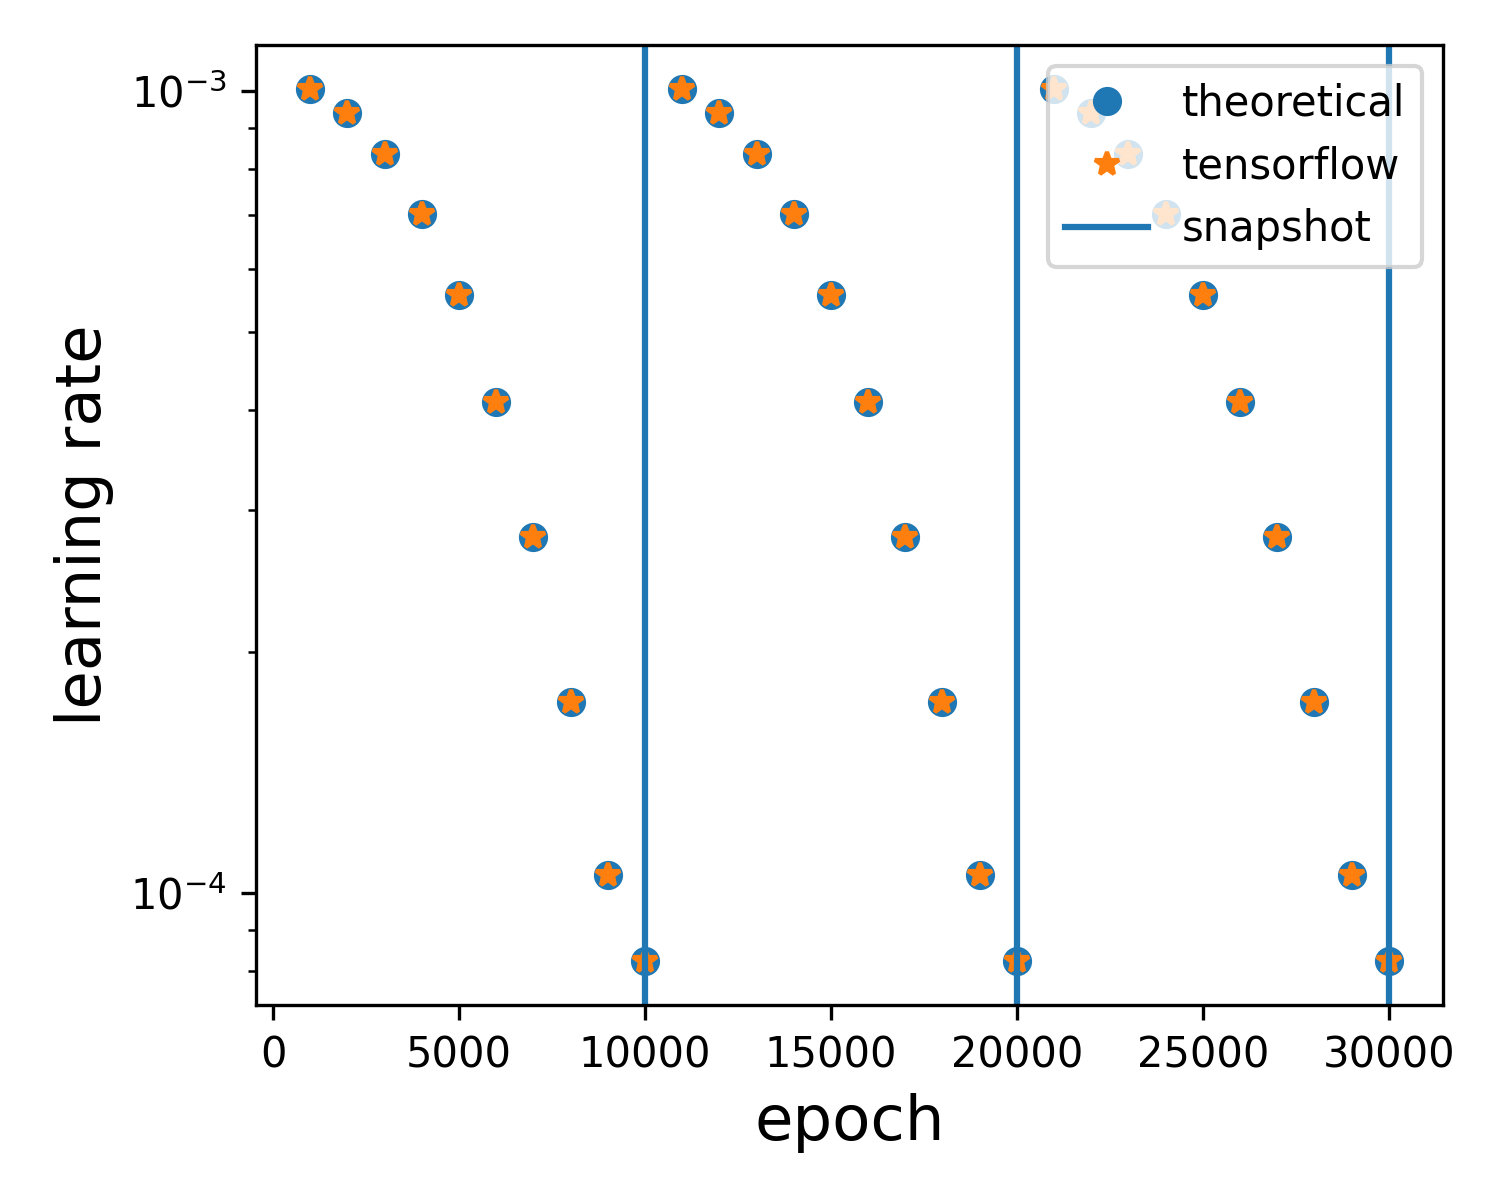
\includegraphics[width=0.6\linewidth]{./figs/learning_schedule.png}  
	\caption{Learning rate schedule: theoretical (SGDR paper) and as computed by tensorflow (sanity check). Snapshot locations also shown (taken before lr restart).}
	\label{fig:lr_sched}
\end{figure}

\newpage
\section{Experiment information}
\noindent
\textbf{True function:}
\begin{equation}
f(x) = 
\begin{cases} 
5 + \sum_{k = 1}^{15} sin(kx) &\text{if } - \pi \leq x < 0\\
cos(10x) & \text{if } 0 \leq x \leq \pi
\end{cases}
\end{equation}
\begin{figure}[H]
	\centering
	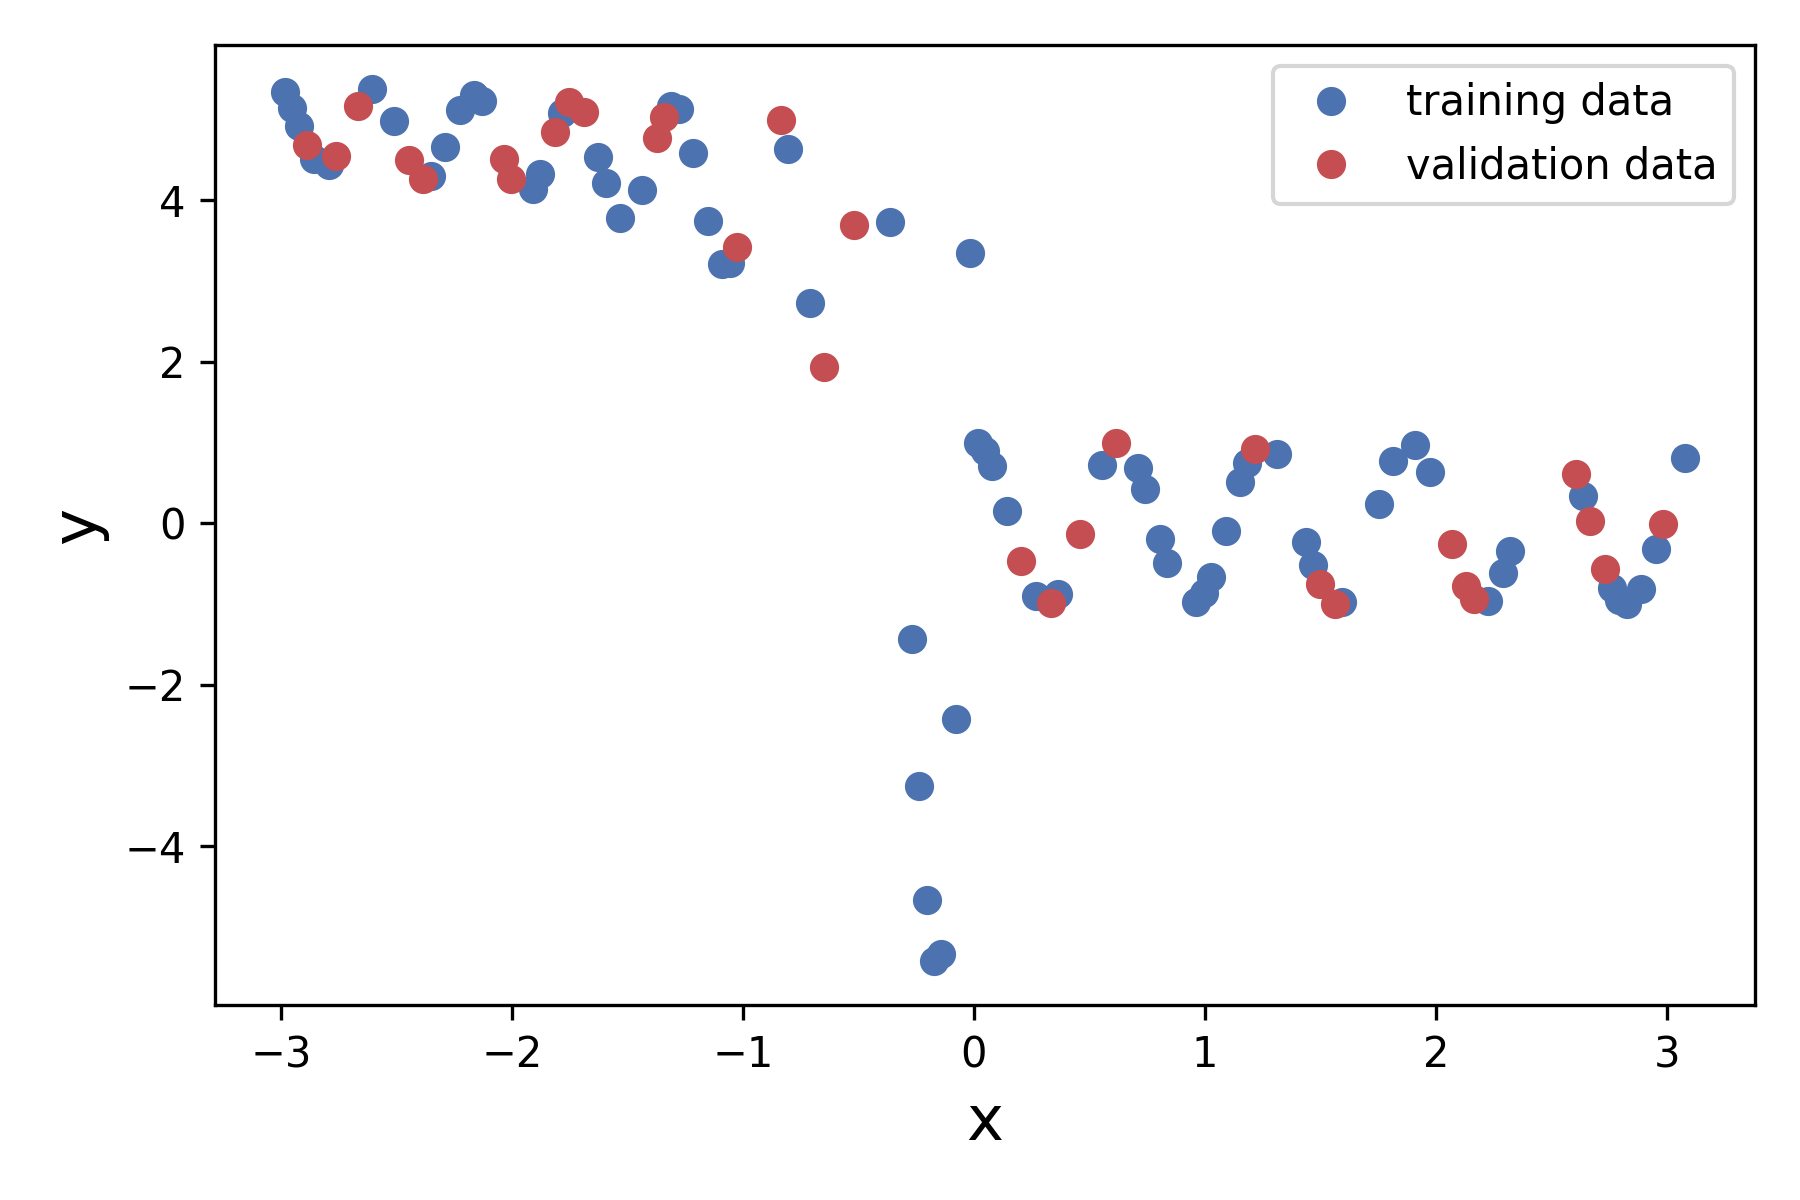
\includegraphics[width=.7\linewidth]{./figs/datapoints.png}  
	\caption{Training and validation data.}
	\label{}
\end{figure}

\noindent
\textbf{Data:}
\begin{center}
	\begin{tabular}{ | c || c |} 
		\hline
		Training datapoints & 70 \\
		\hline
		Validation datapoints & 30 \\
		\hline
		Noise std & 0 \\
		\hline
		Evaluation datapoints & 200 \\
		\hline
	\end{tabular}
\end{center}


\noindent
\textbf{What we want to see:}
\begin{itemize}
	\item Snapshots should give low error predictions and diverse; i.e., with high point-wise standard deviation.
	\item When ensembled, the final predictions should give a better test error compared to a single model.
	\item Uncertainty should be higher at the locations of large error. Predictions should agree on over-specified areas and disagree on under-specified ones.
	\item Snapshot ensembles (1 trajectory) are expected to be less accurate than deep ensembles (many trajectories). 
	\item Snapshots with constant learning rate should be less diverse than snapshots with cosine annealing and restarts.
	\item But snapshots with cosine annealing are expected to be less diverse than deep ensembles.	
\end{itemize}

\noindent
\textbf{Architecture and hyperparameters:}
\begin{center}
	\begin{tabular}{ | c || c| c|} 
		\hline
		 & Standard lr & Cosine annealing	\\
		\hline
		Depth & \multicolumn{2}{c|}{5*} \\
		\hline
		Width  & \multicolumn{2}{c|}{49*} \\
		\hline
		Max budget (epochs)& \multicolumn{2}{c|}{60,000} \\
		\hline
		Optimizer& \multicolumn{2}{c|}{Adam} \\
		\hline
		Initializer& \multicolumn{2}{c|}{Xavier} \\
		\hline
		Repetitions& \multicolumn{2}{c|}{6} \\
		\hline
		Number of cycles (if not varying) &  NA & 6\\ 
		\hline
		Snapshot step (if not varying) & NA  & $10,000$\\ 
		\hline
		Number of snapshots (if not varying) &  NA  & 6\\ 
		\hline
		Constant lr & 4e-4* & NA\\ 
		\hline
		Cosine annealing min lr & NA & 8e-5**\\ 
		\hline
		Cosine annealing max lr & NA & 1e-3**\\ 
		\hline
	\end{tabular}
\end{center}
\noindent *: obtained via random search \\
\noindent **: obtained via random search with fixed architecture

\section{Figures}

\begin{figure}[H]
	\begin{subfigure}[b]{.45\textwidth}
		\centering
		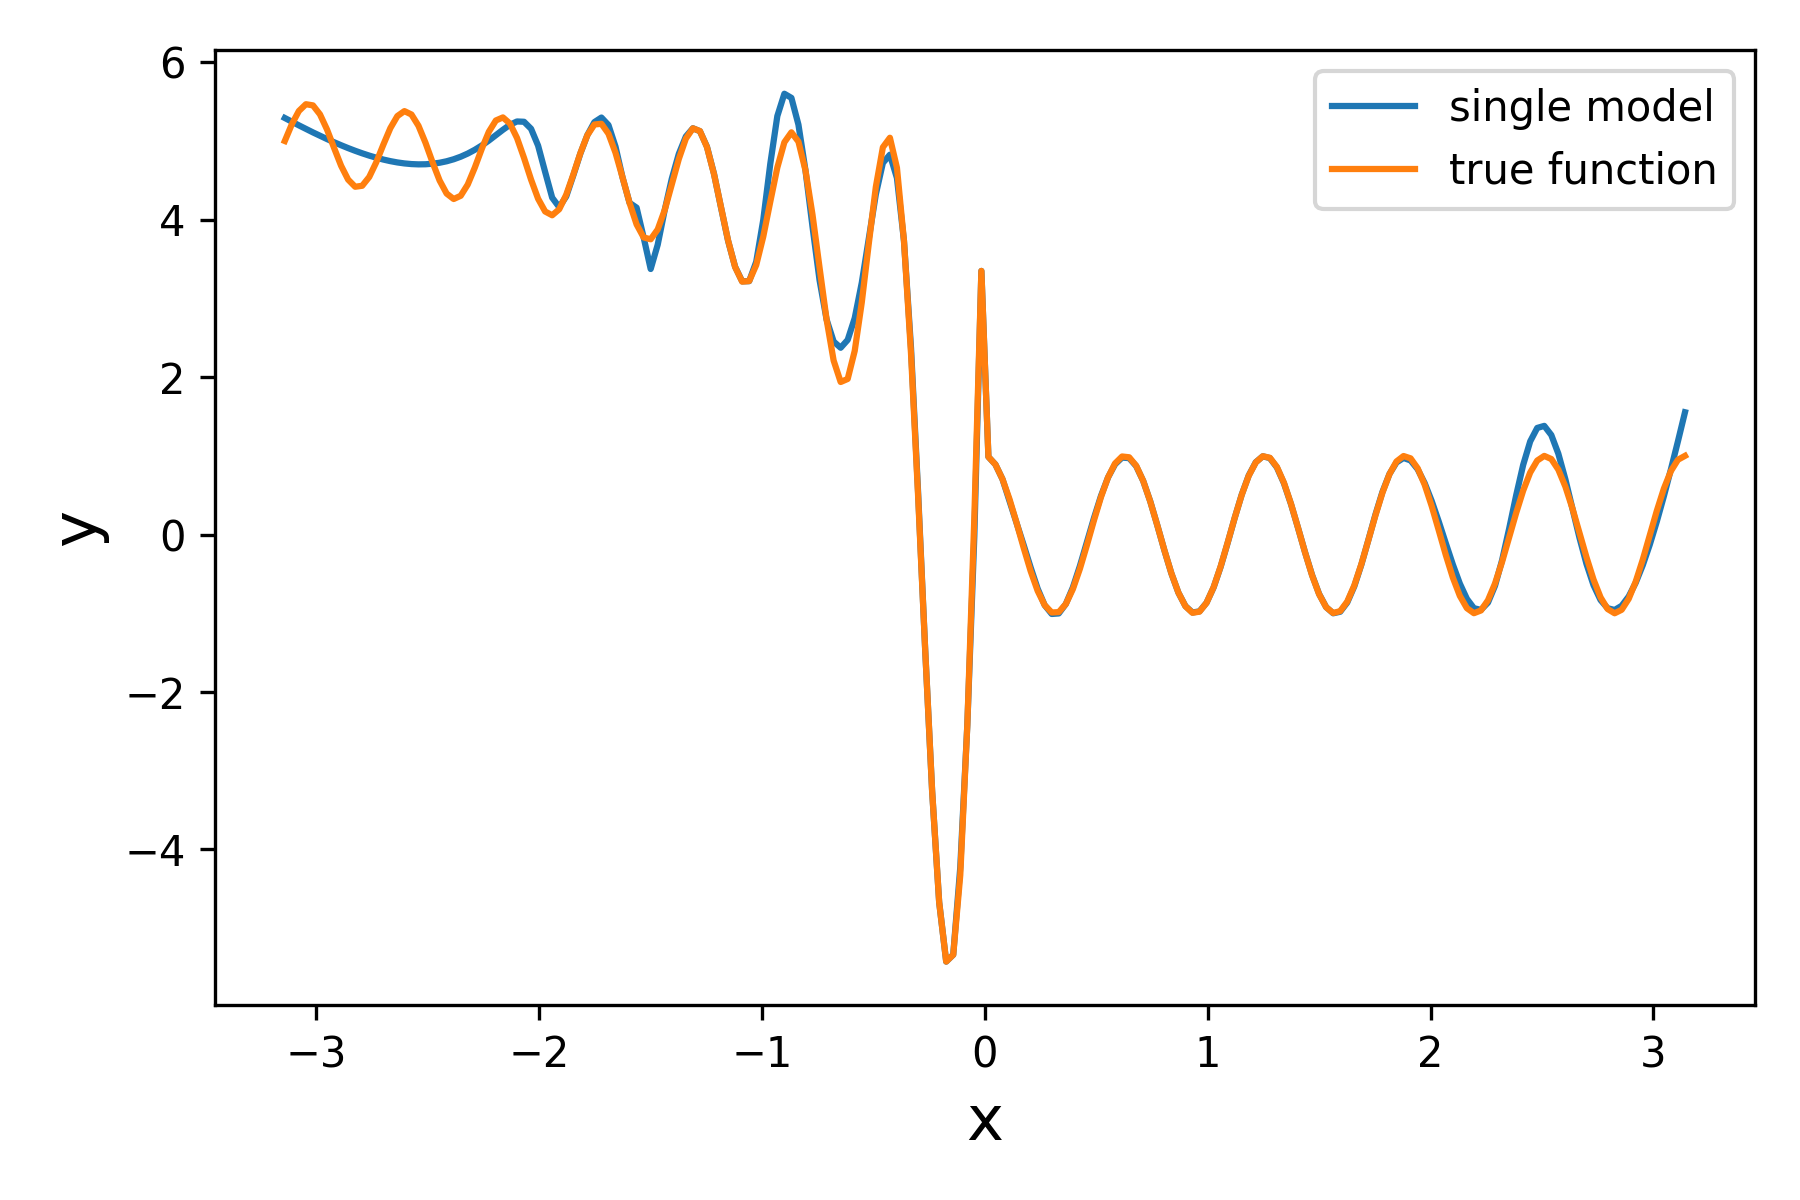
\includegraphics[width=1\linewidth]{./figs/sm_rep_fun.png}  
		\caption{Single model: A representative predicted function.}
	\end{subfigure}
	\begin{subfigure}[b]{.45\textwidth}
		\centering
		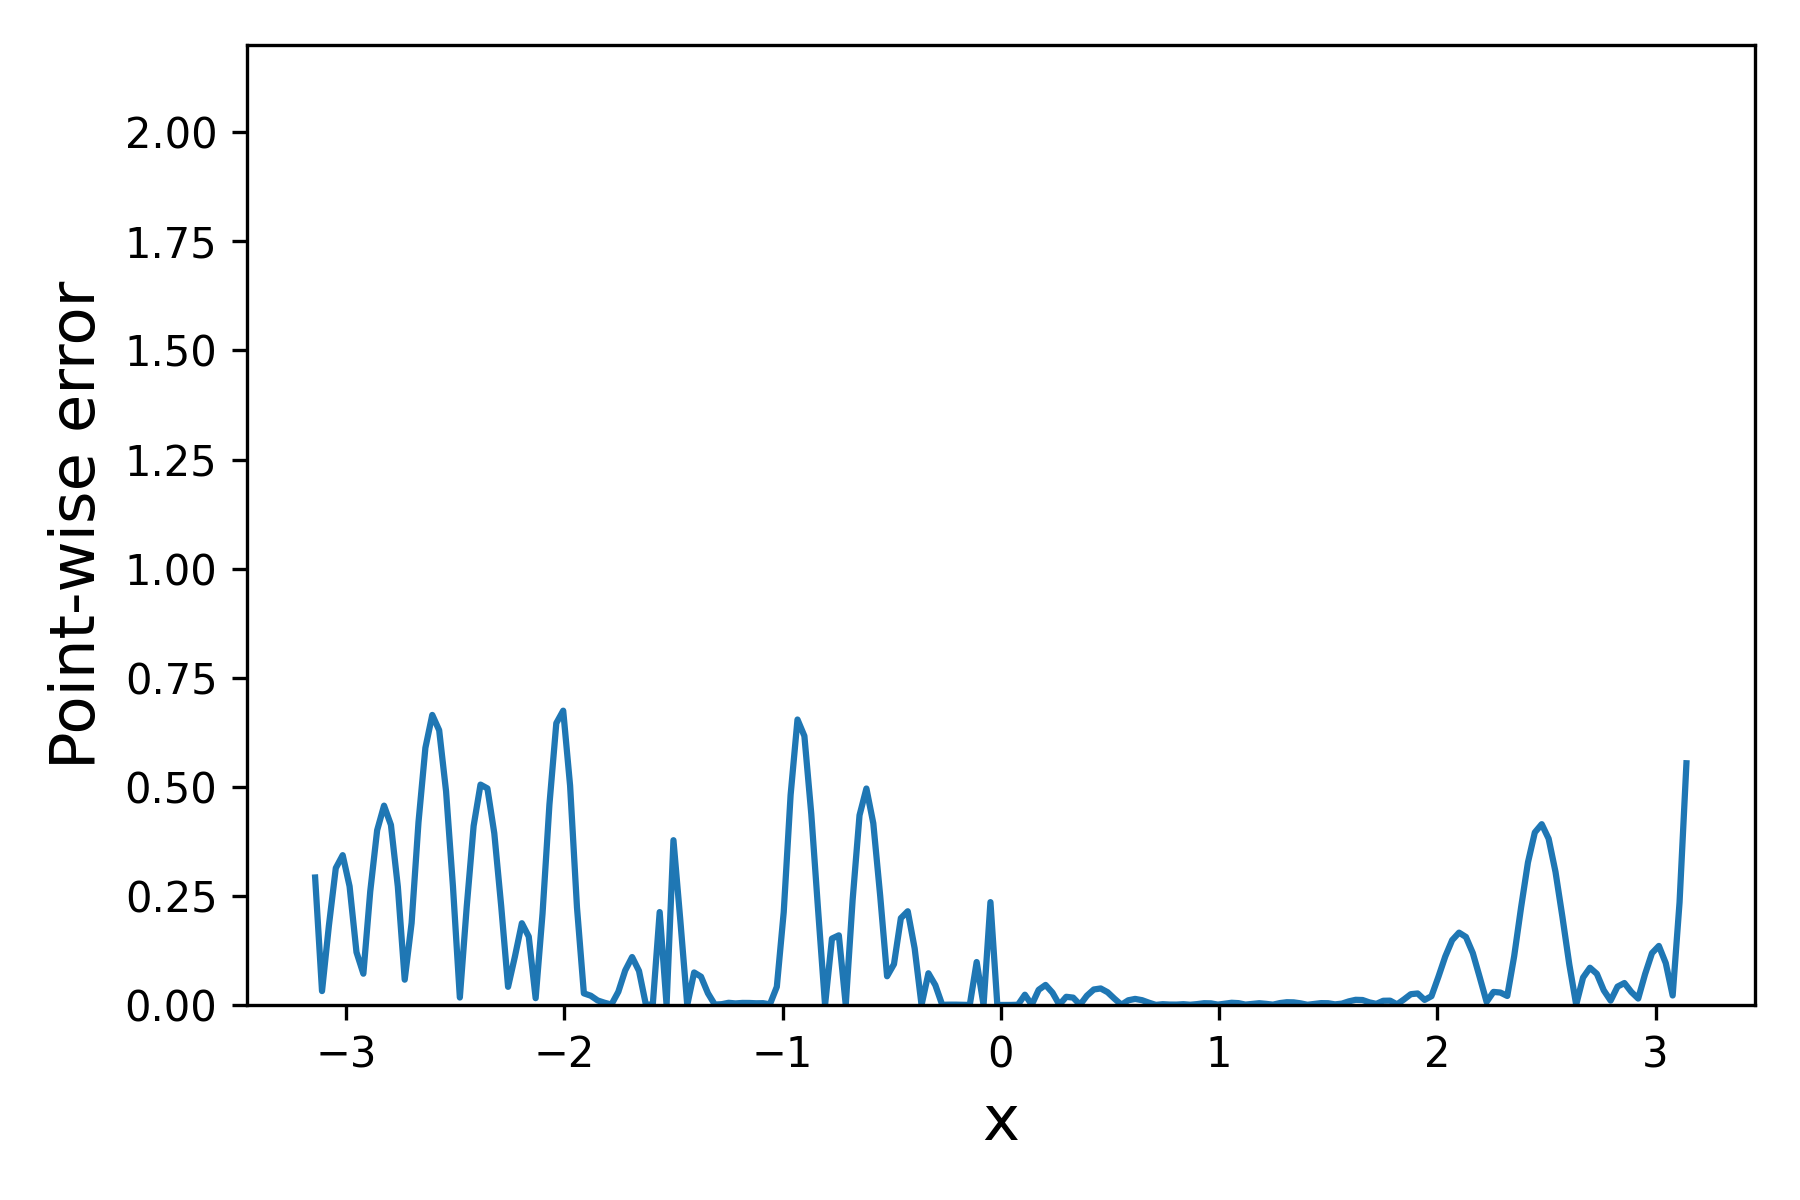
\includegraphics[width=1\linewidth]{./figs/sm_rep_err.png}  
		\caption{Single model: Associated point-wise error.}
	\end{subfigure}
	\begin{subfigure}[b]{.45\textwidth}
		\centering
		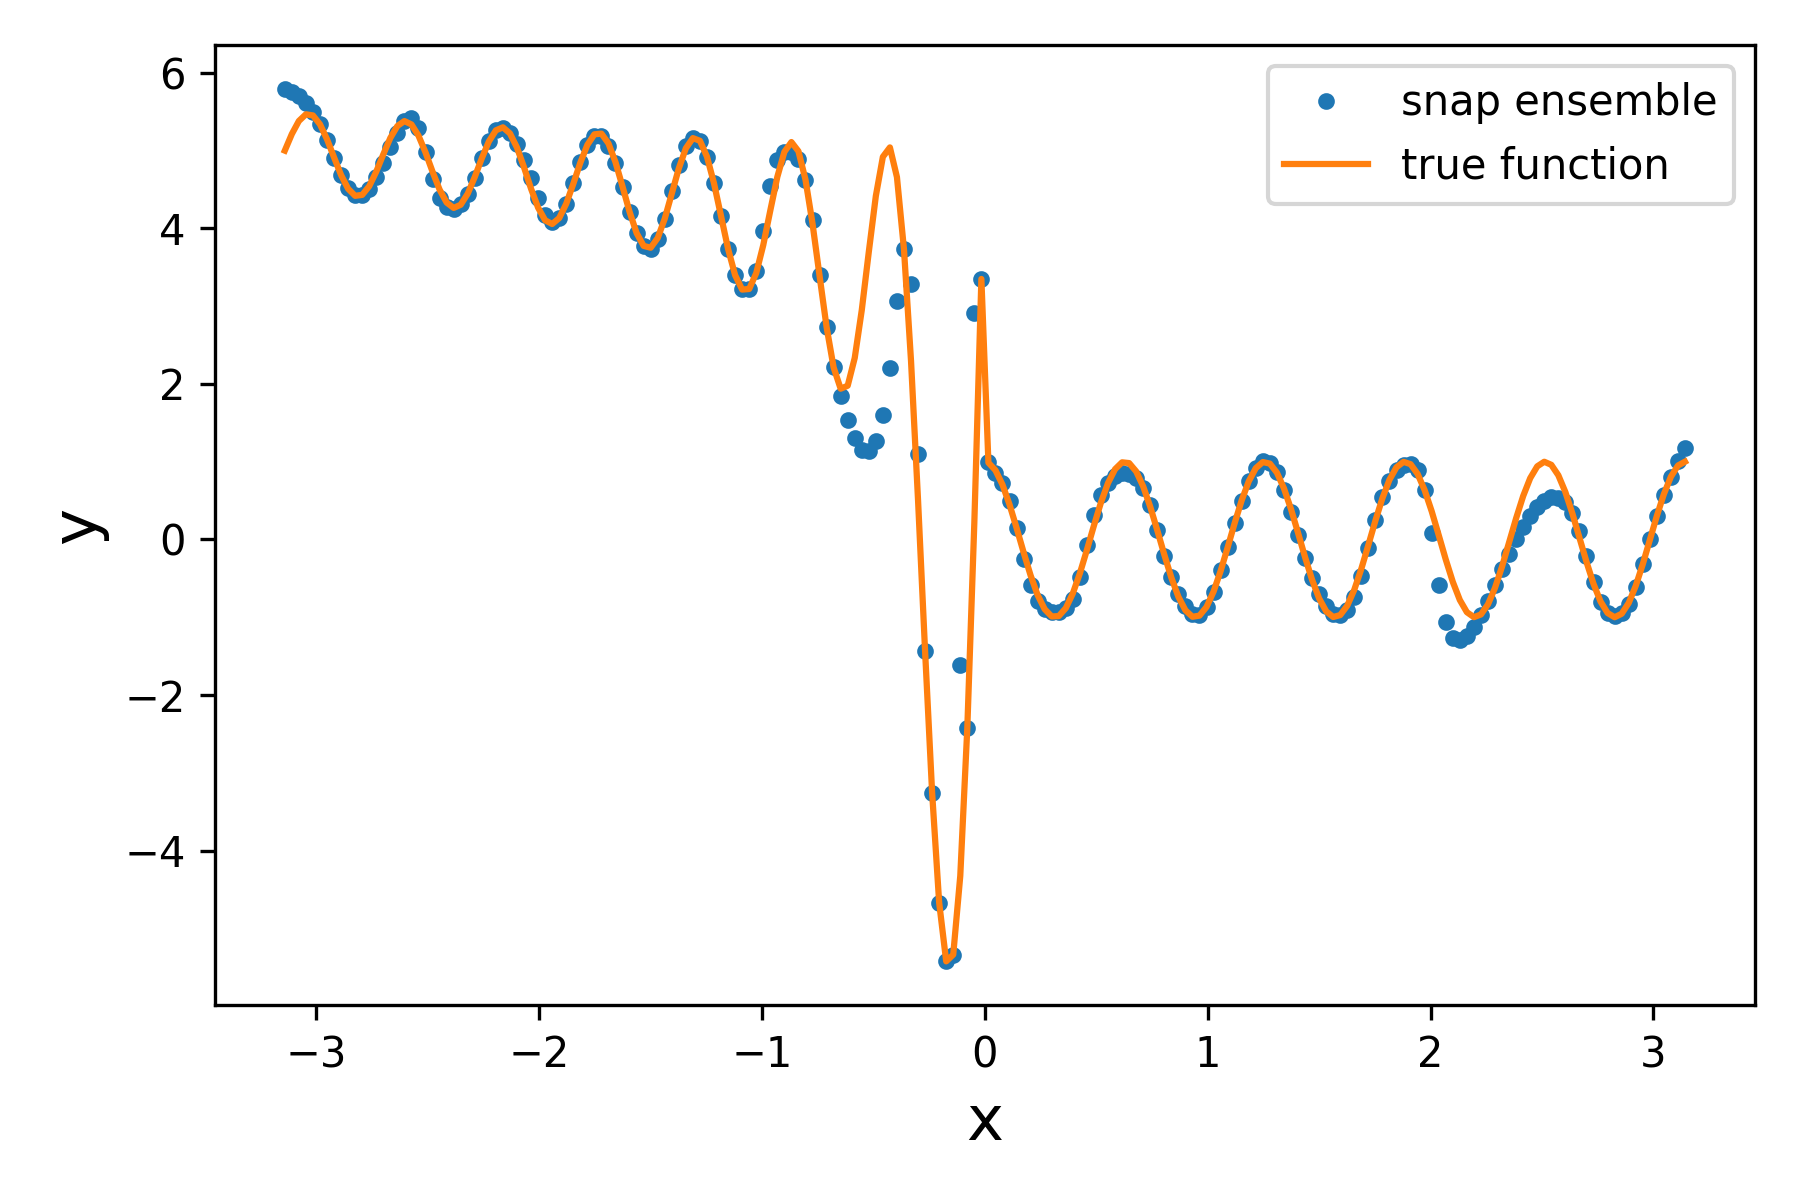
\includegraphics[width=1\linewidth]{./figs/snap_rep_fun.png}  
		\caption{Snapshot ensemble: A representative predicted function $\pm 2$ stds.
		Uncertainty estimates obtained via snapshots of a single trajectory.}
	\end{subfigure}
	\begin{subfigure}[b]{.45\textwidth}
		\centering
		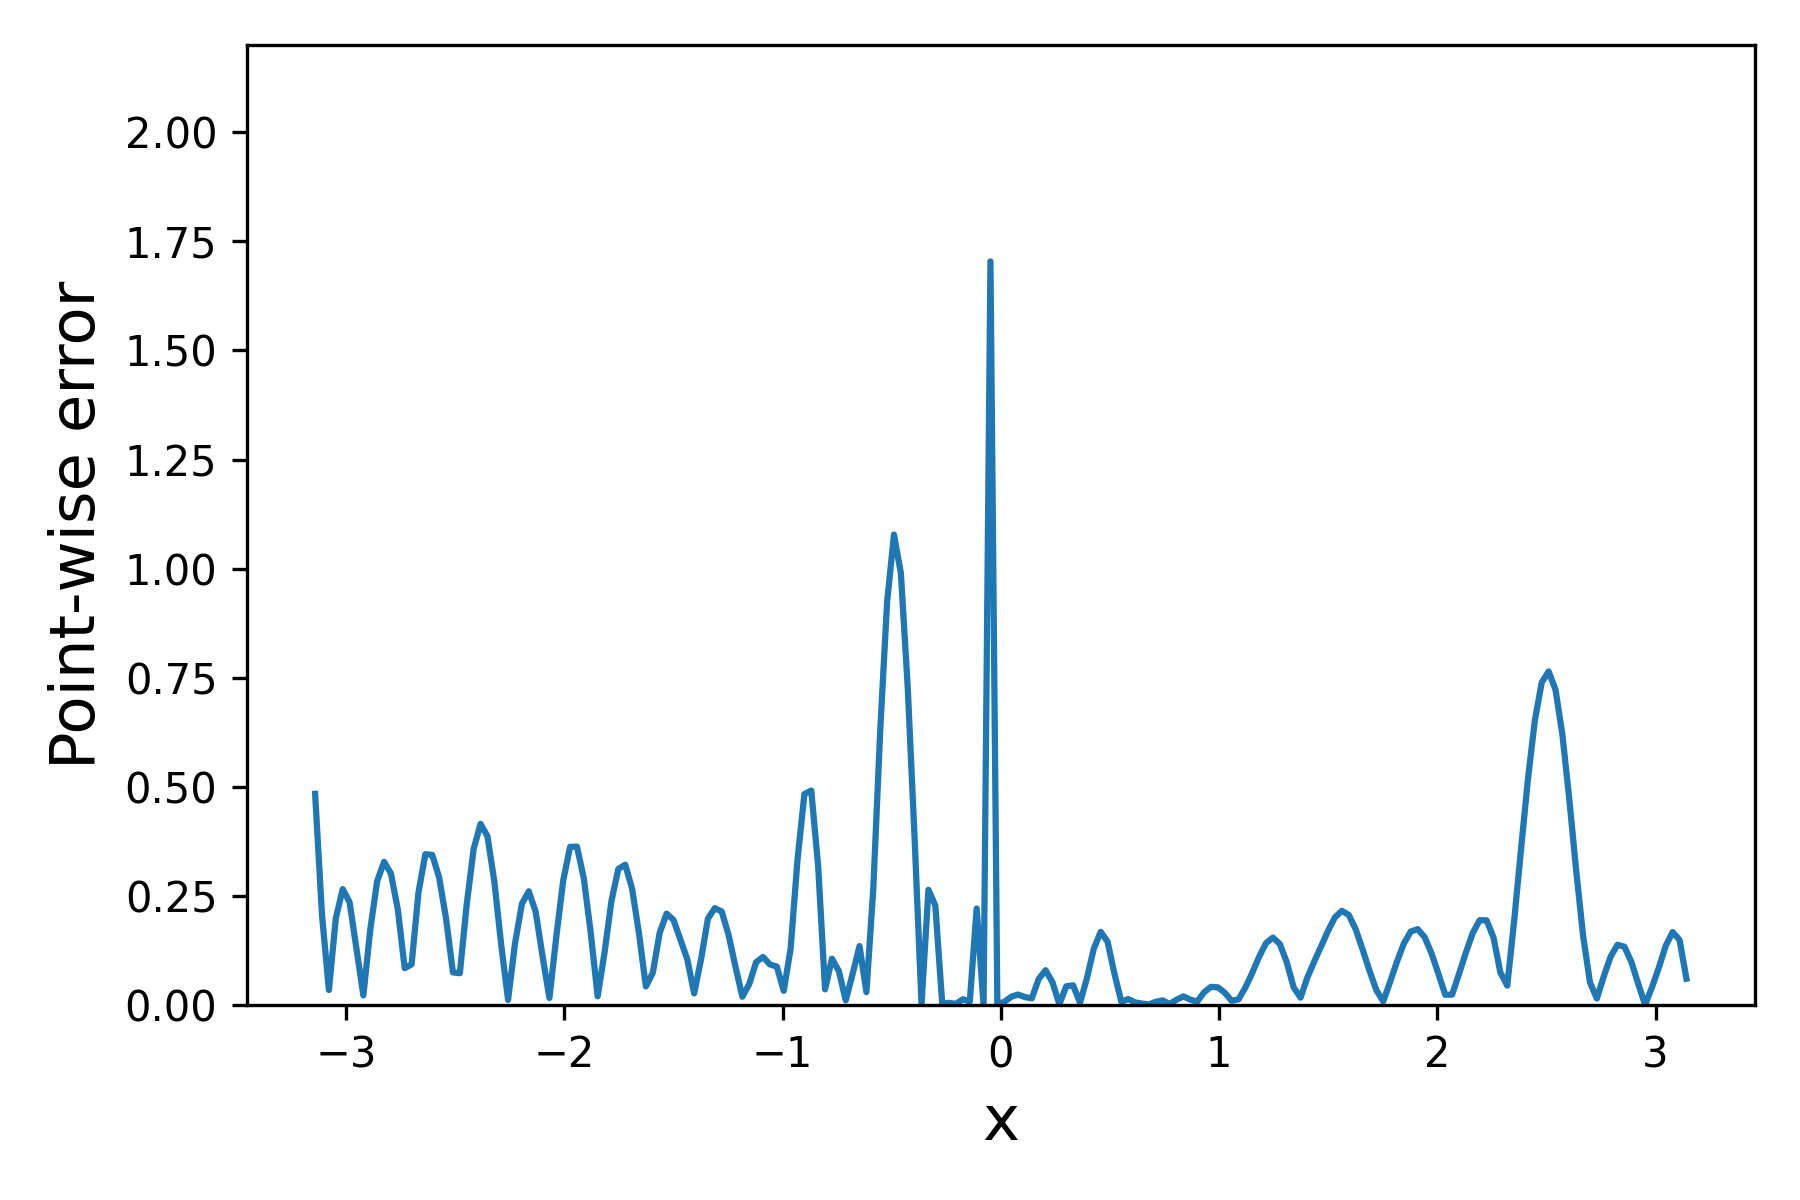
\includegraphics[width=1\linewidth]{./figs/snap_rep_err.png}  
		\caption{Snapshot ensemble: Associated point-wise error. \newline \newline}
	\end{subfigure}
	\begin{subfigure}[b]{.45\textwidth}
		\centering
		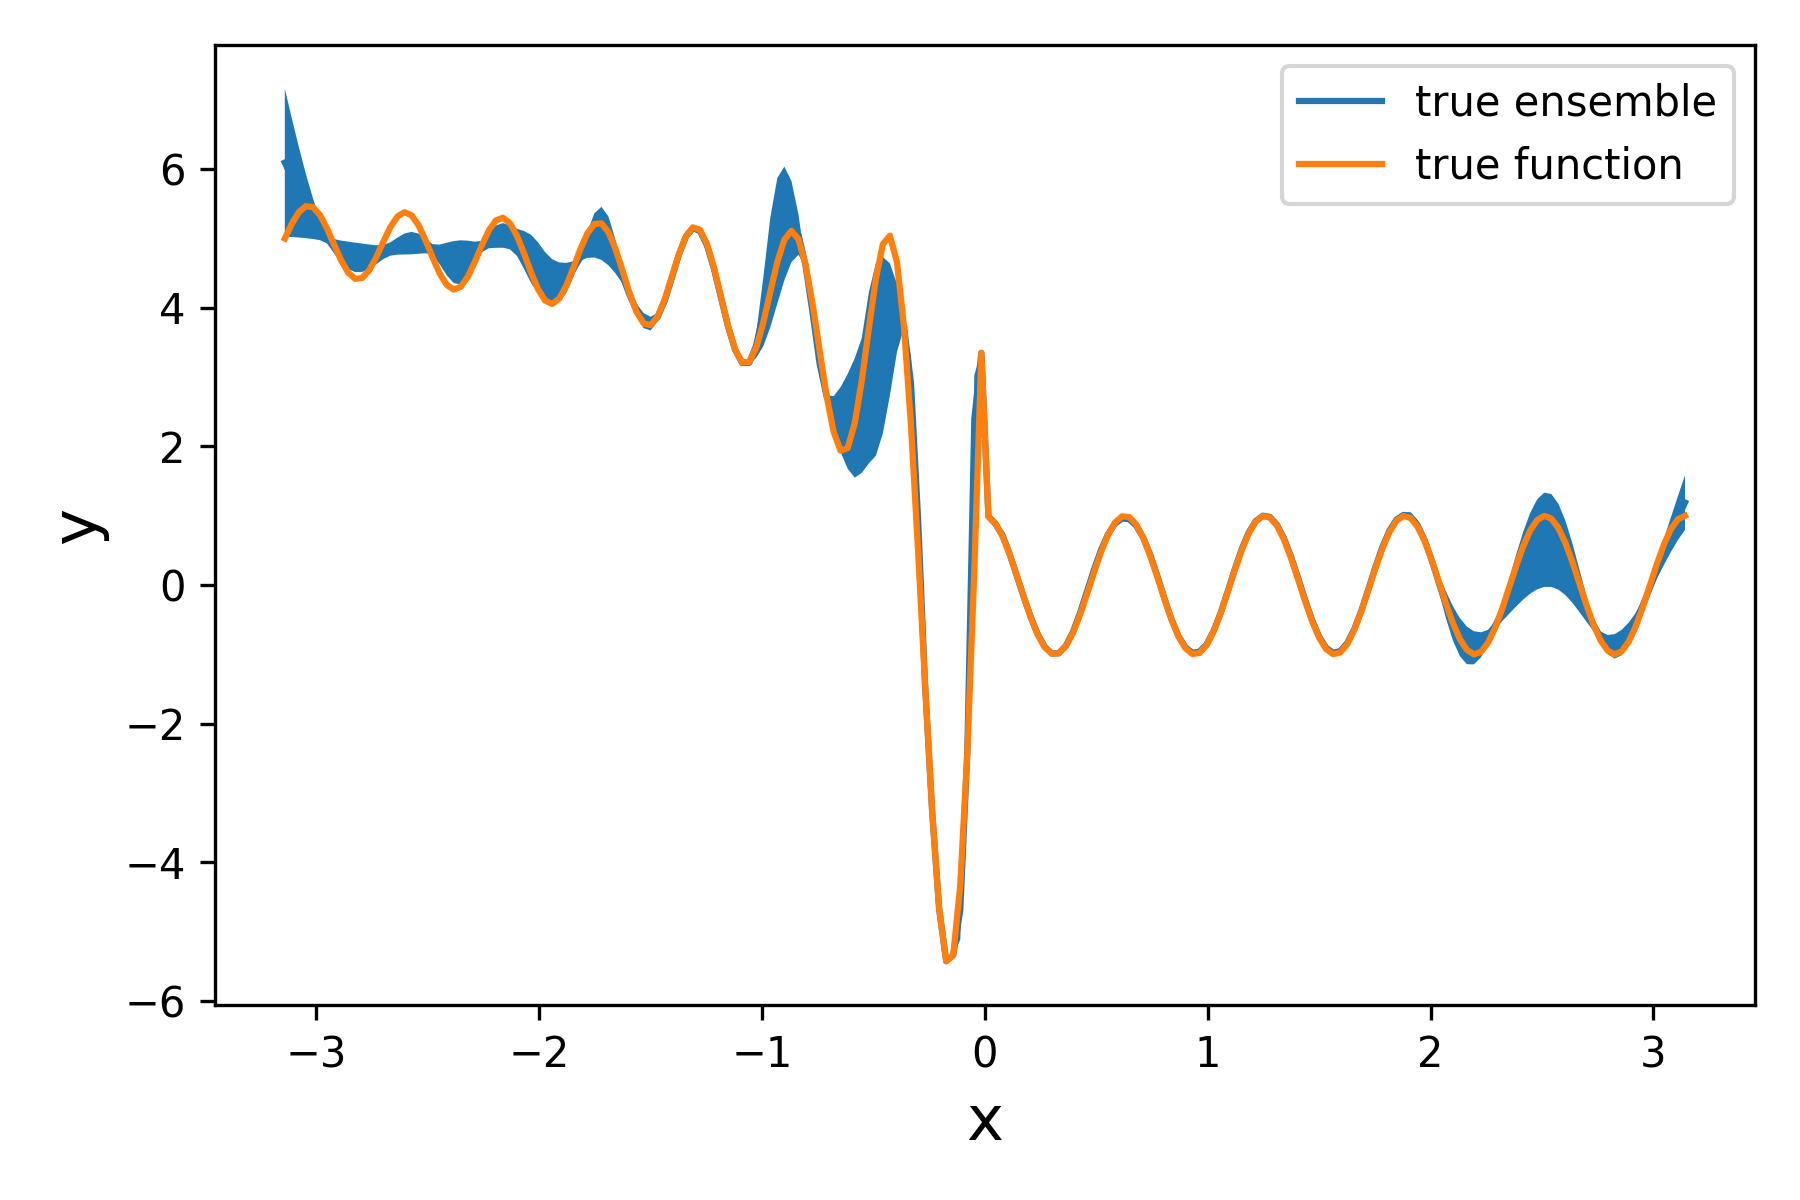
\includegraphics[width=1\linewidth]{./figs/ens_rep_fun.png}  
		\caption{True ensemble: A representative predicted function $\pm 2$ stds.
		Uncertainty estimates obtained via different trajectories.}
	\end{subfigure}
	\hspace{1cm}
	\begin{subfigure}[b]{.45\textwidth}
		\centering
		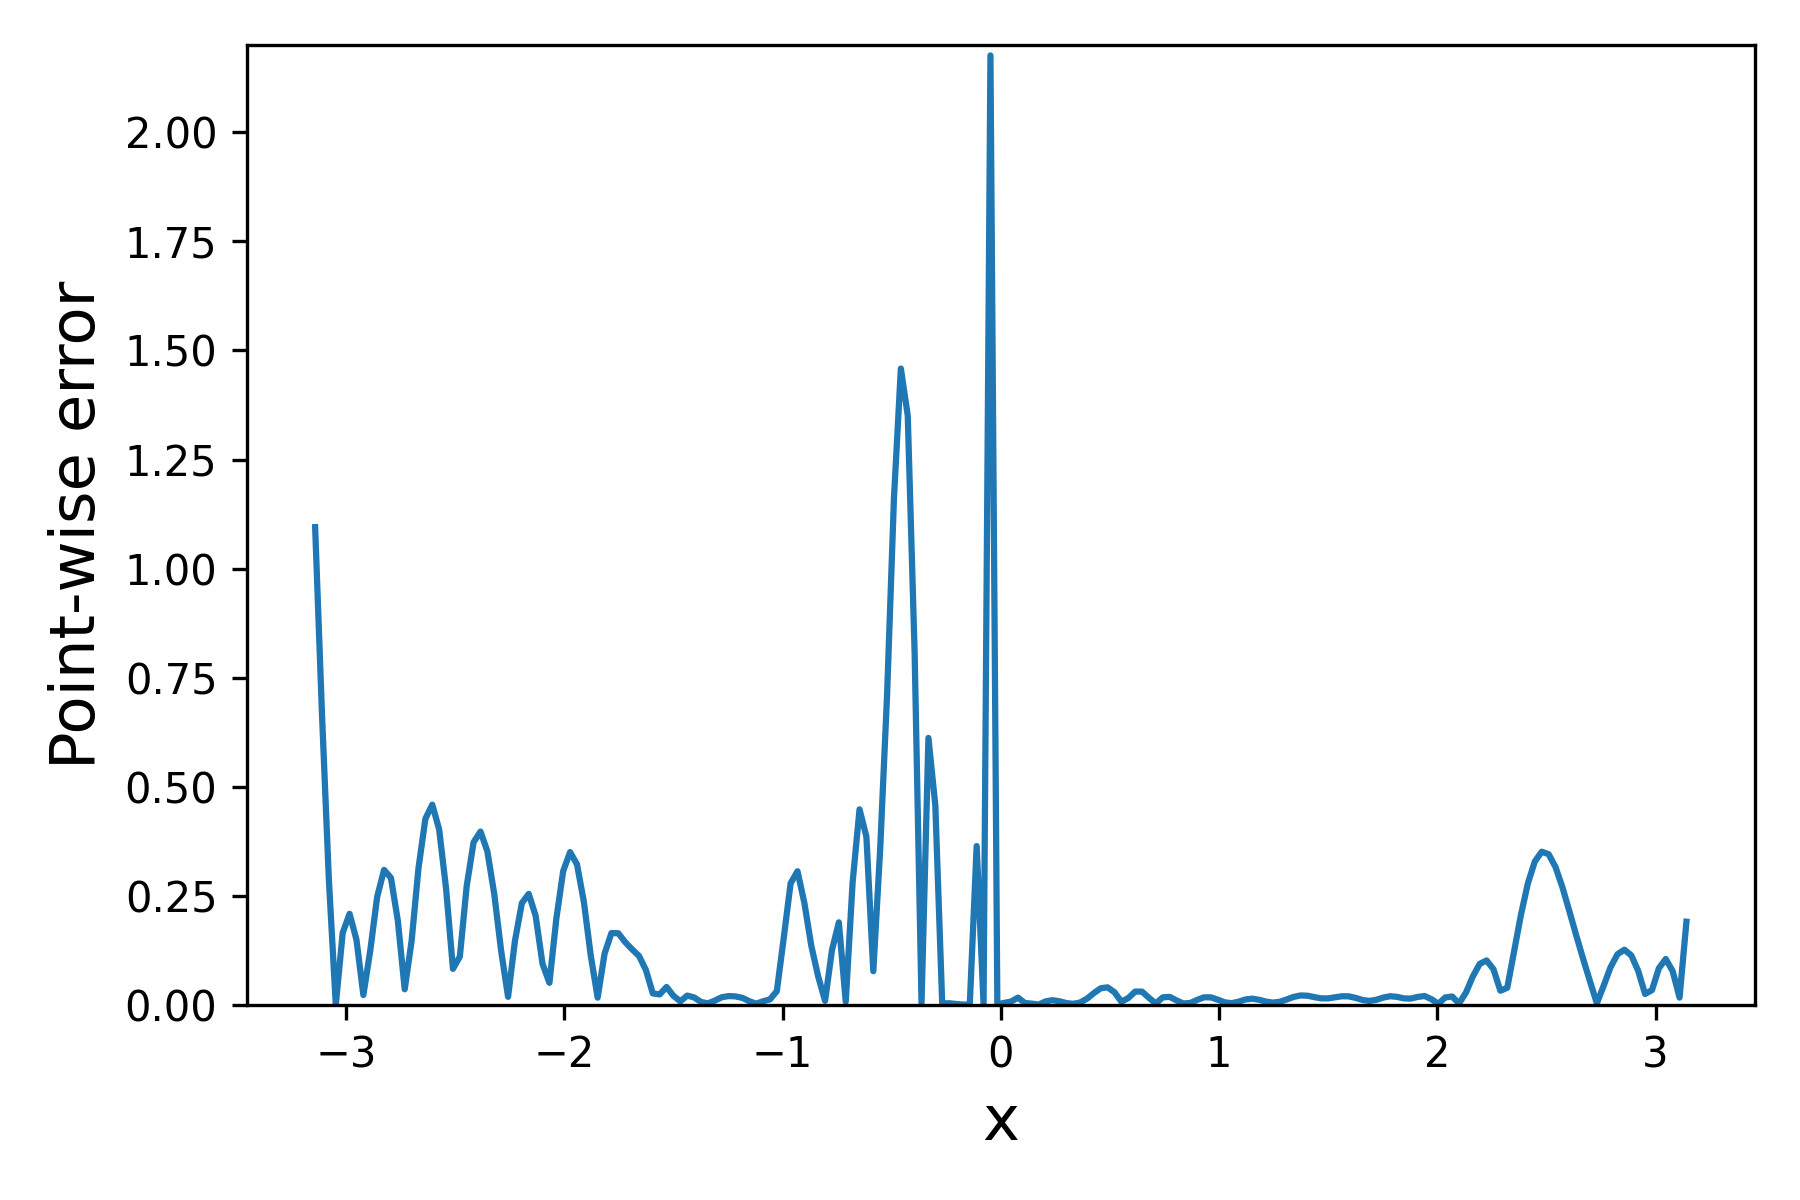
\includegraphics[width=1\linewidth]{./figs/ens_rep_err.png}  
		\caption{True ensemble: Associated point-wise error. \newline}
	\end{subfigure}
	\caption{Representative predicted functions, uncertainty estimates and point-wise errors for a single model, a snapshot ensemble and a true ensemble.}
\end{figure}

\begin{figure}[H]
	\begin{subfigure}[b]{.45\textwidth}
		\centering
		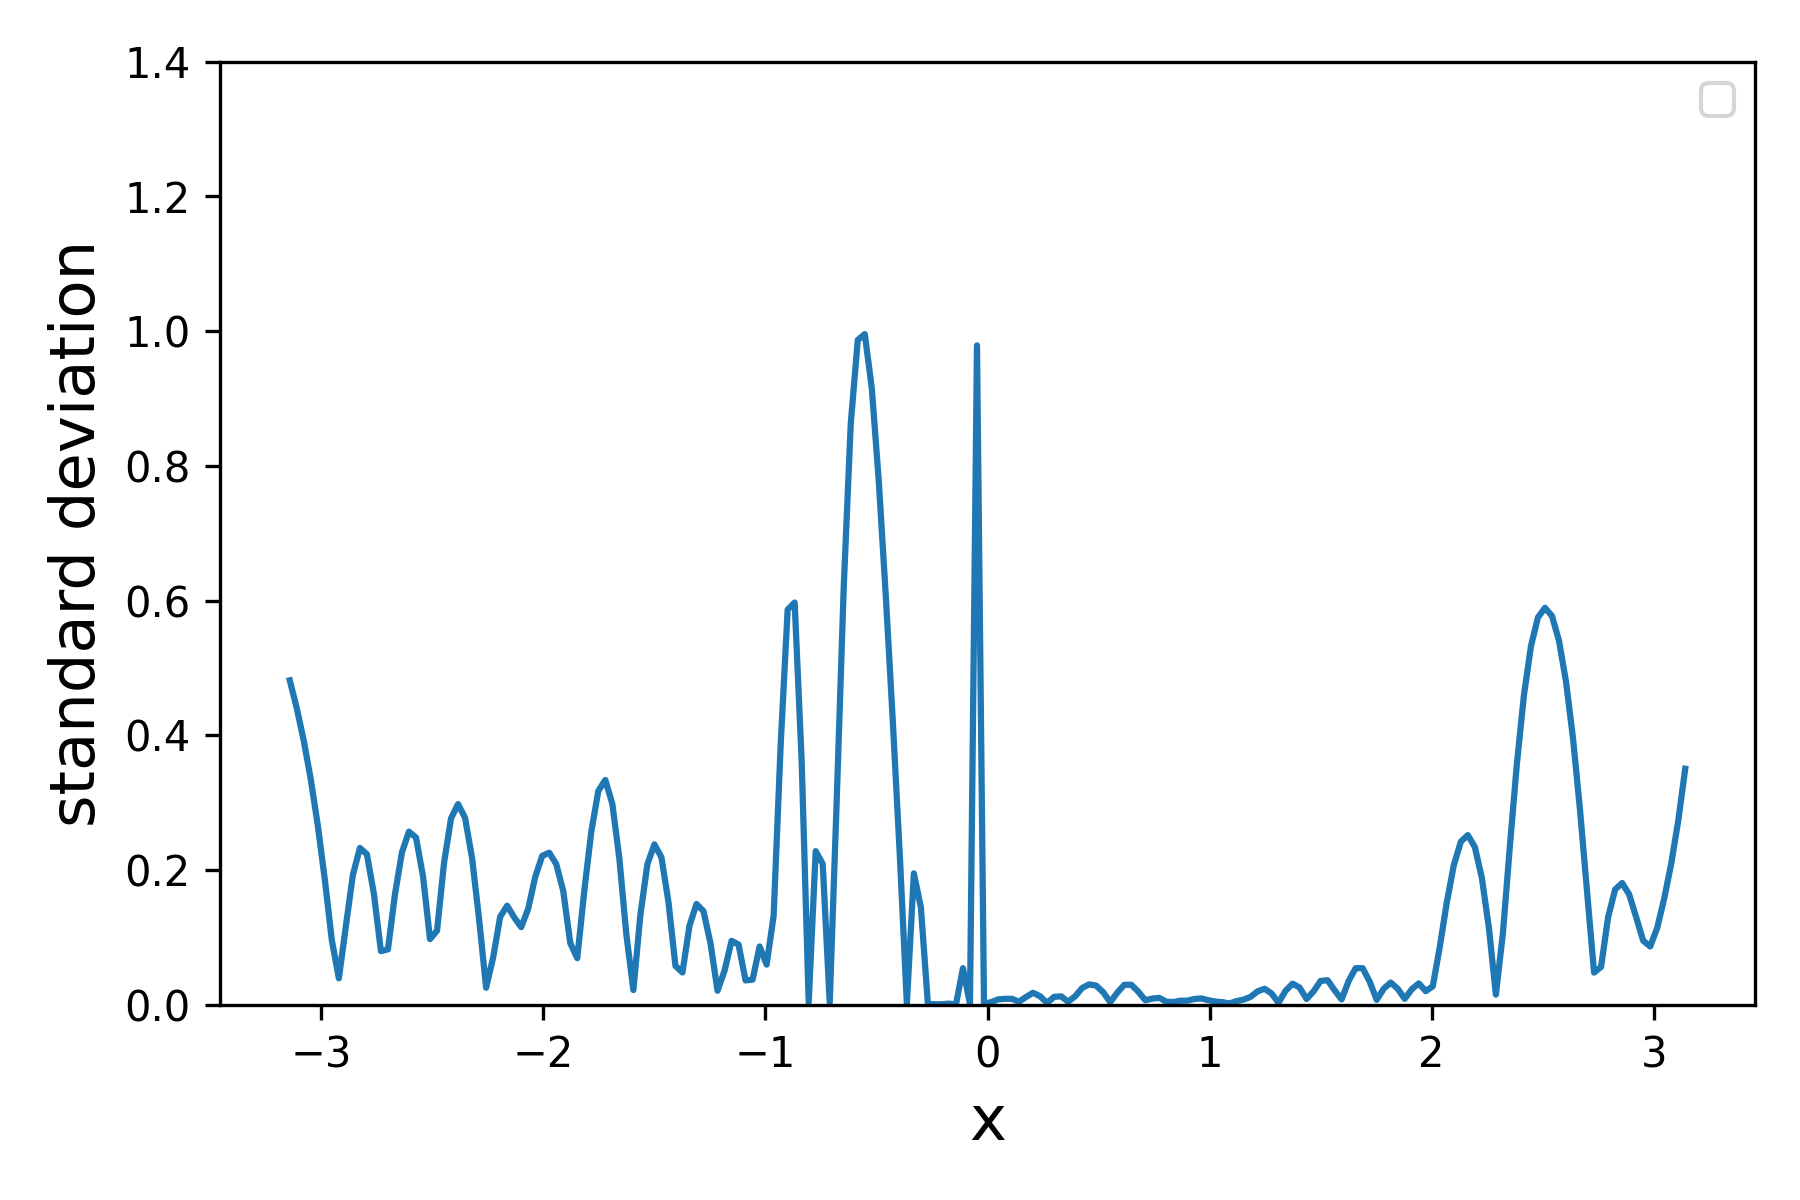
\includegraphics[width=1\linewidth]{./figs/snap_rep_std.png}  
		\caption{Snapshot ensemble: Standard deviation of predicted functions corresponding to snapshots from 1 trajectory.}
	\end{subfigure}
	\begin{subfigure}[b]{.45\textwidth}
		\centering
		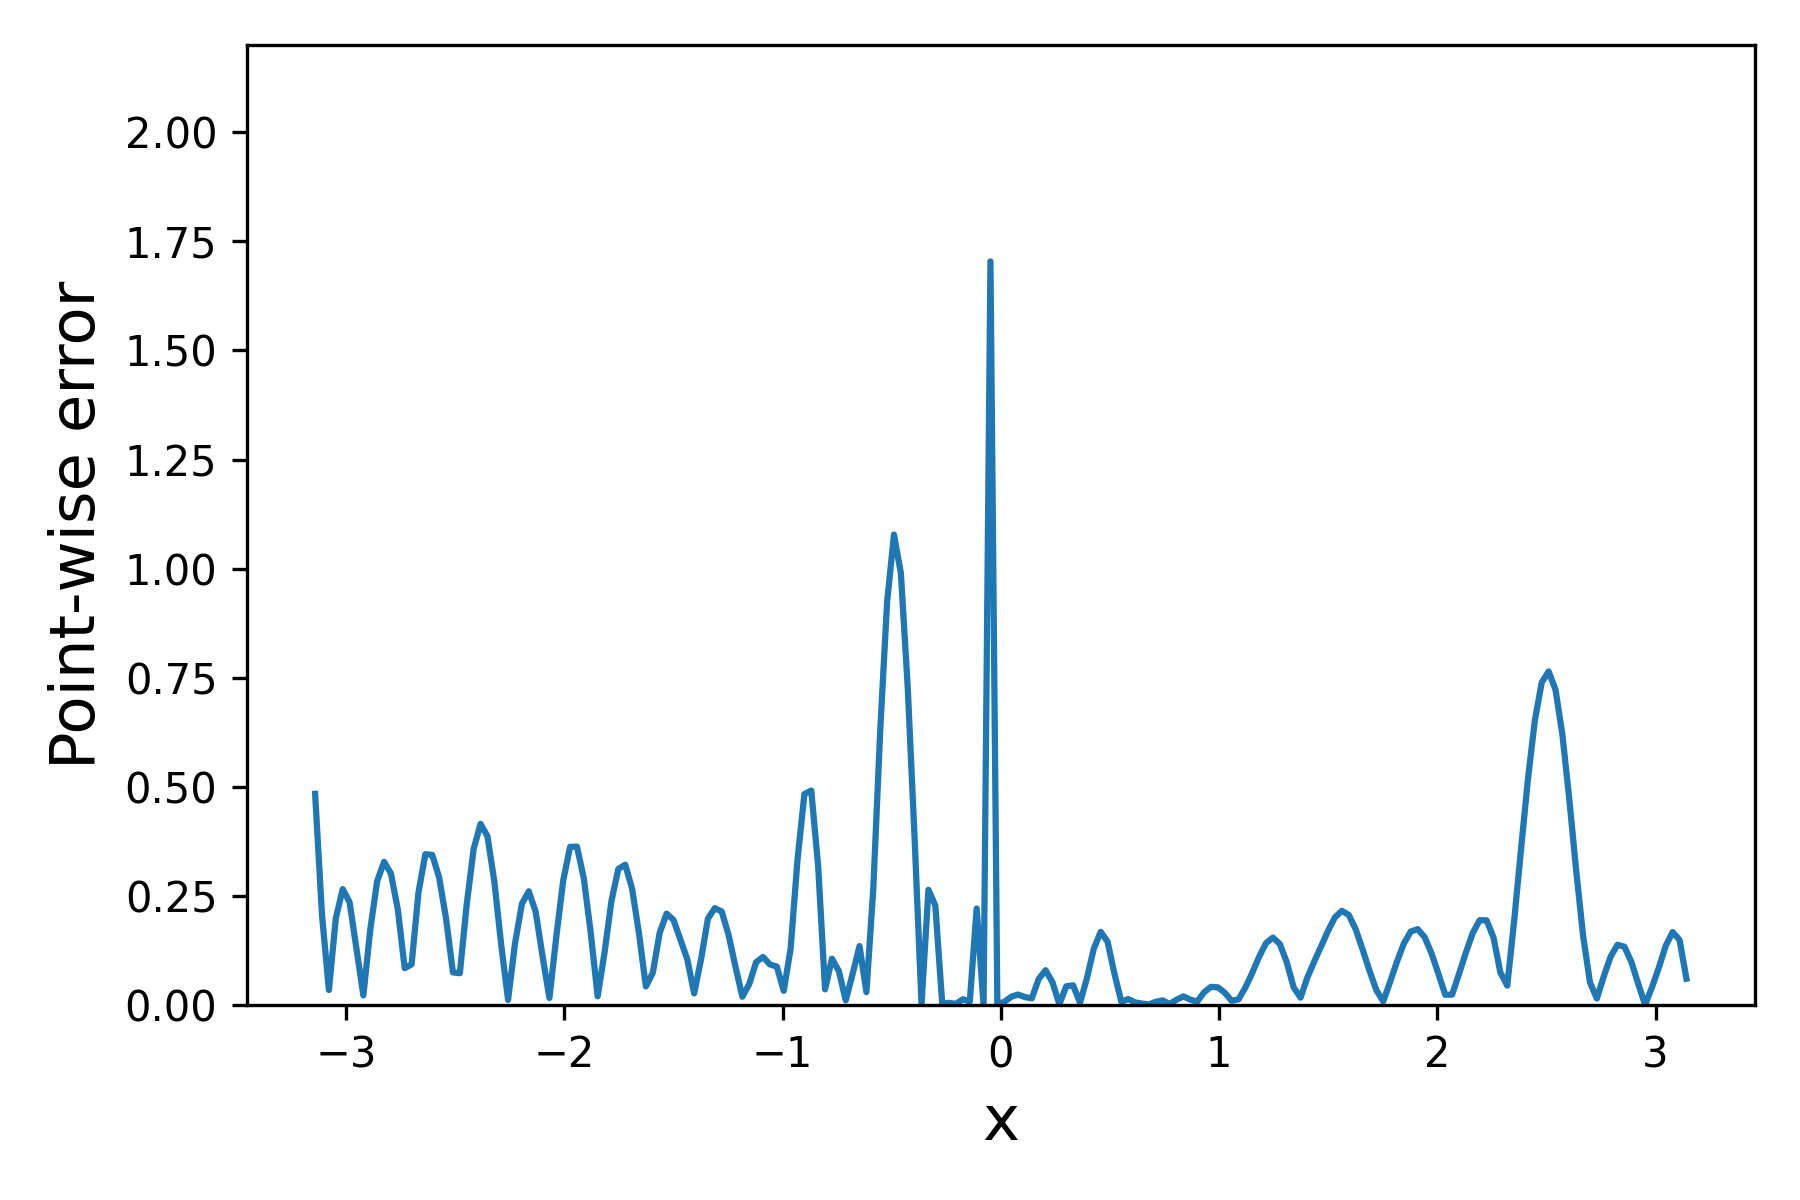
\includegraphics[width=1\linewidth]{./figs/snap_rep_err.png}  
		\caption{Snapshot ensemble: Associated point-wise error. \newline}
	\end{subfigure}
	\begin{subfigure}[b]{.45\textwidth}
		\centering
		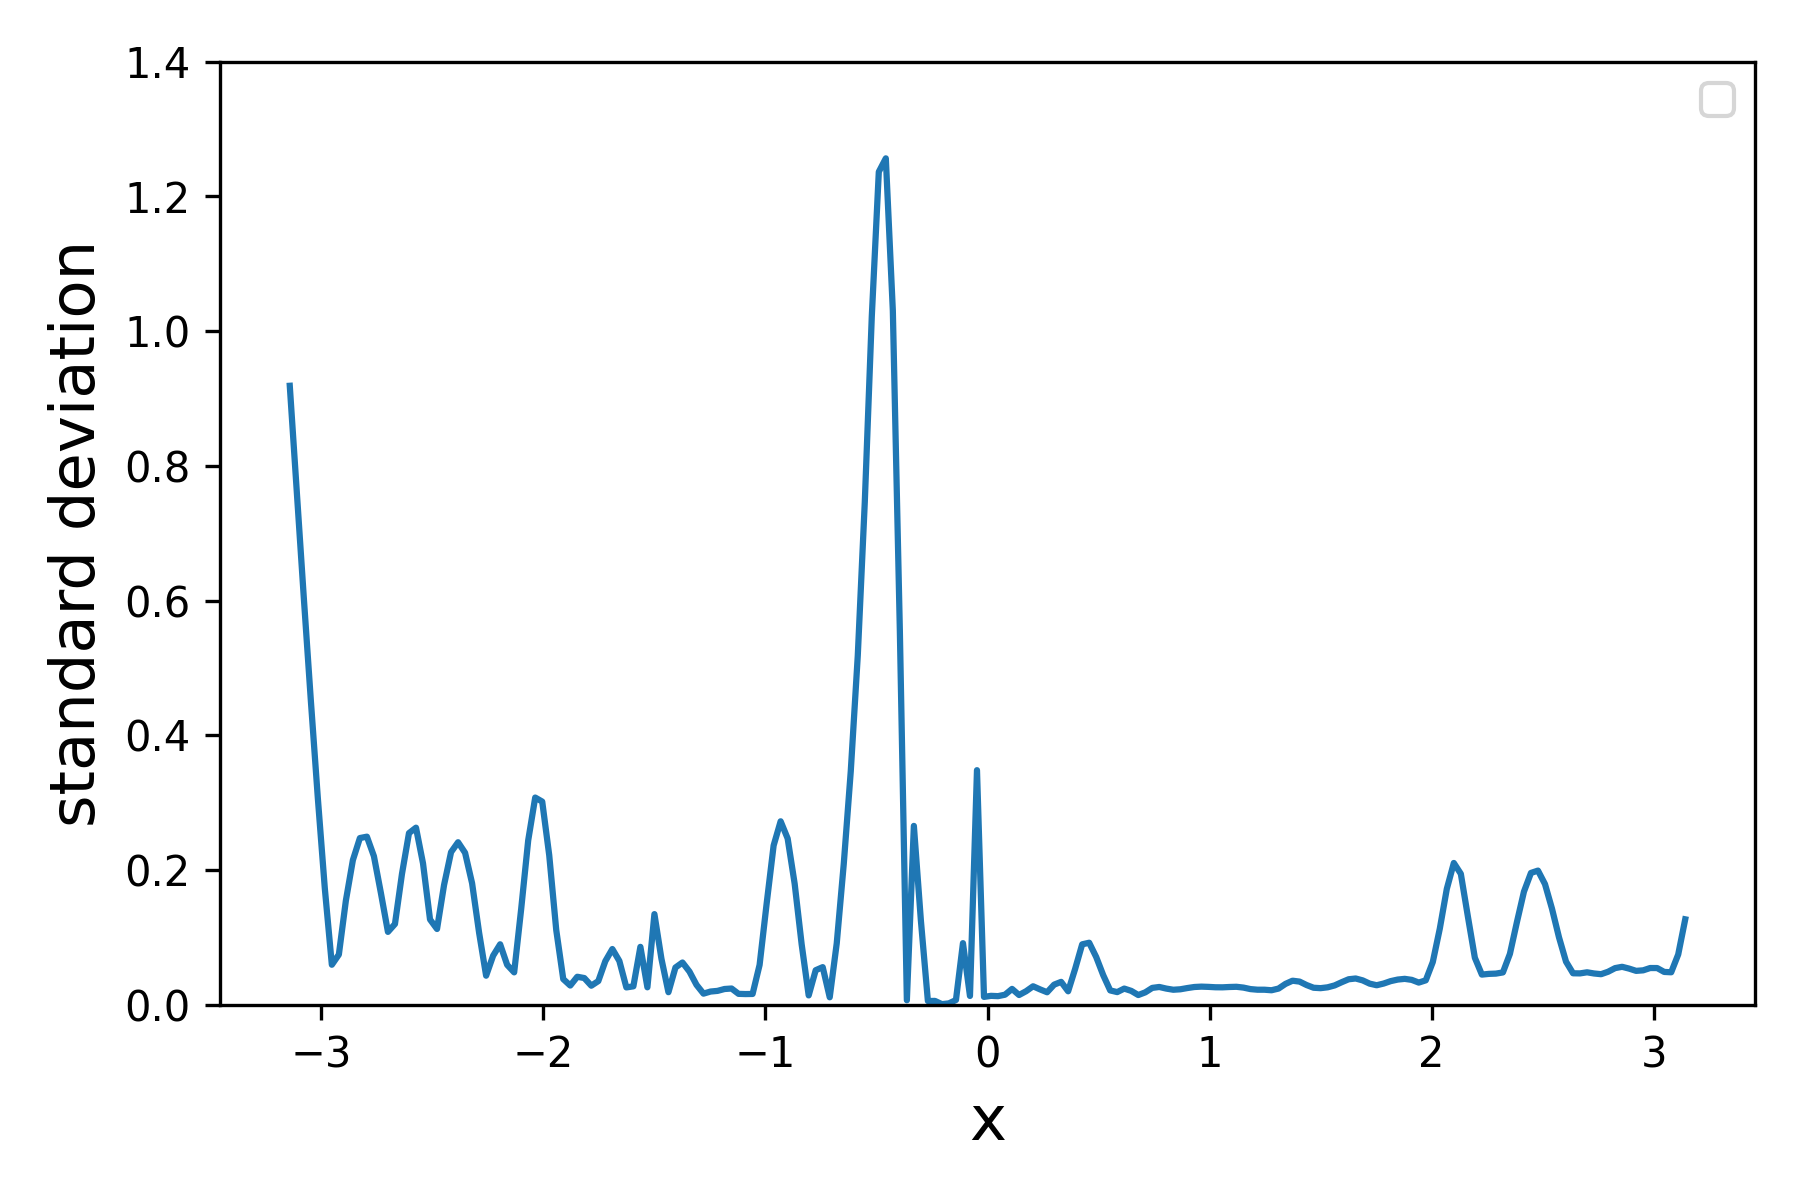
\includegraphics[width=1\linewidth]{./figs/ens_std.png}  
		\caption{True ensemble: Standard deviation of predicted functions corresponding to final parameters from different trajectories.}
	\end{subfigure}
	\hspace{1cm}
	\begin{subfigure}[b]{.45\textwidth}
		\centering
		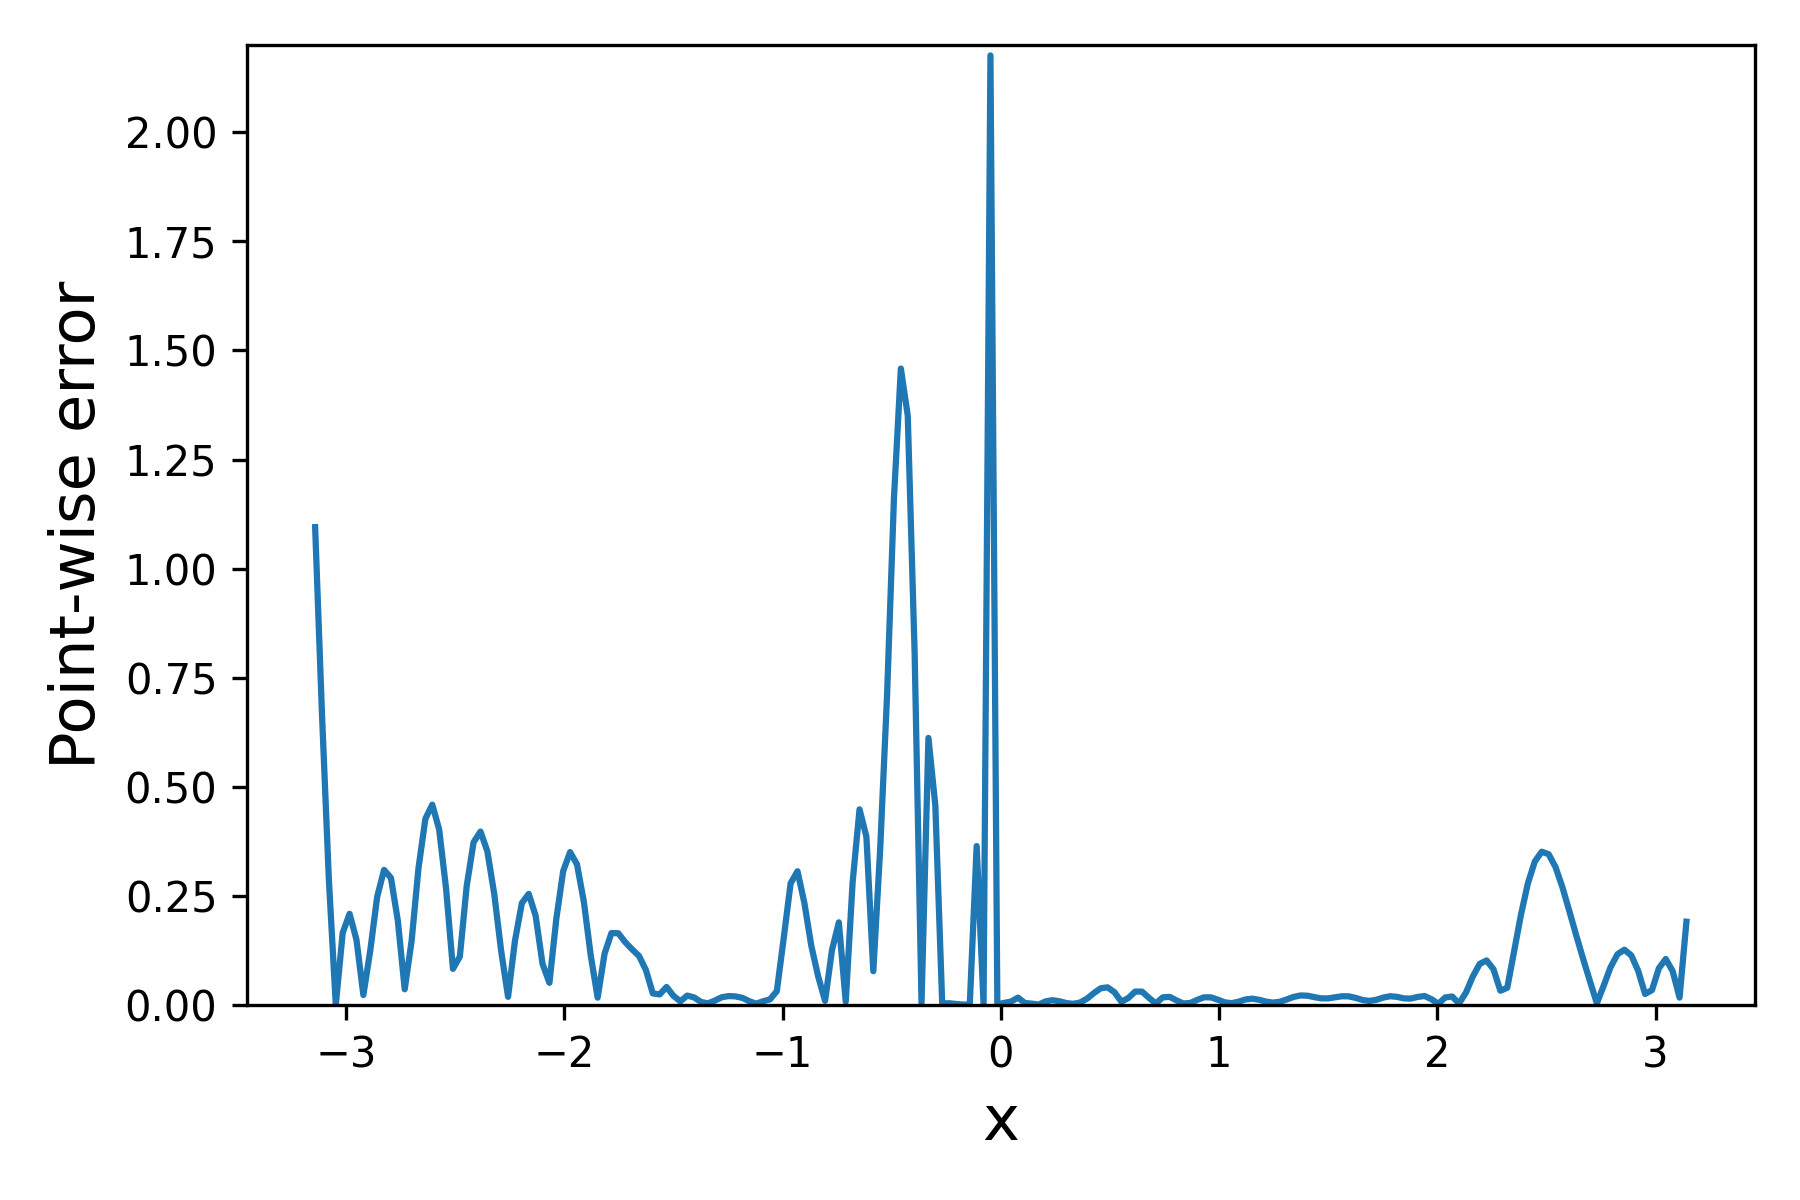
\includegraphics[width=1\linewidth]{./figs/ens_rep_err.png}  
		\caption{True ensemble: Associated point-wise error. \newline}
	\end{subfigure}
	\caption{Representative uncertainty estimates and point-wise errors for a snapshot ensemble and a true ensemble.}
\end{figure}

\begin{figure}[H]
	\centering
	\begin{subfigure}{.45\textwidth}
		\centering
		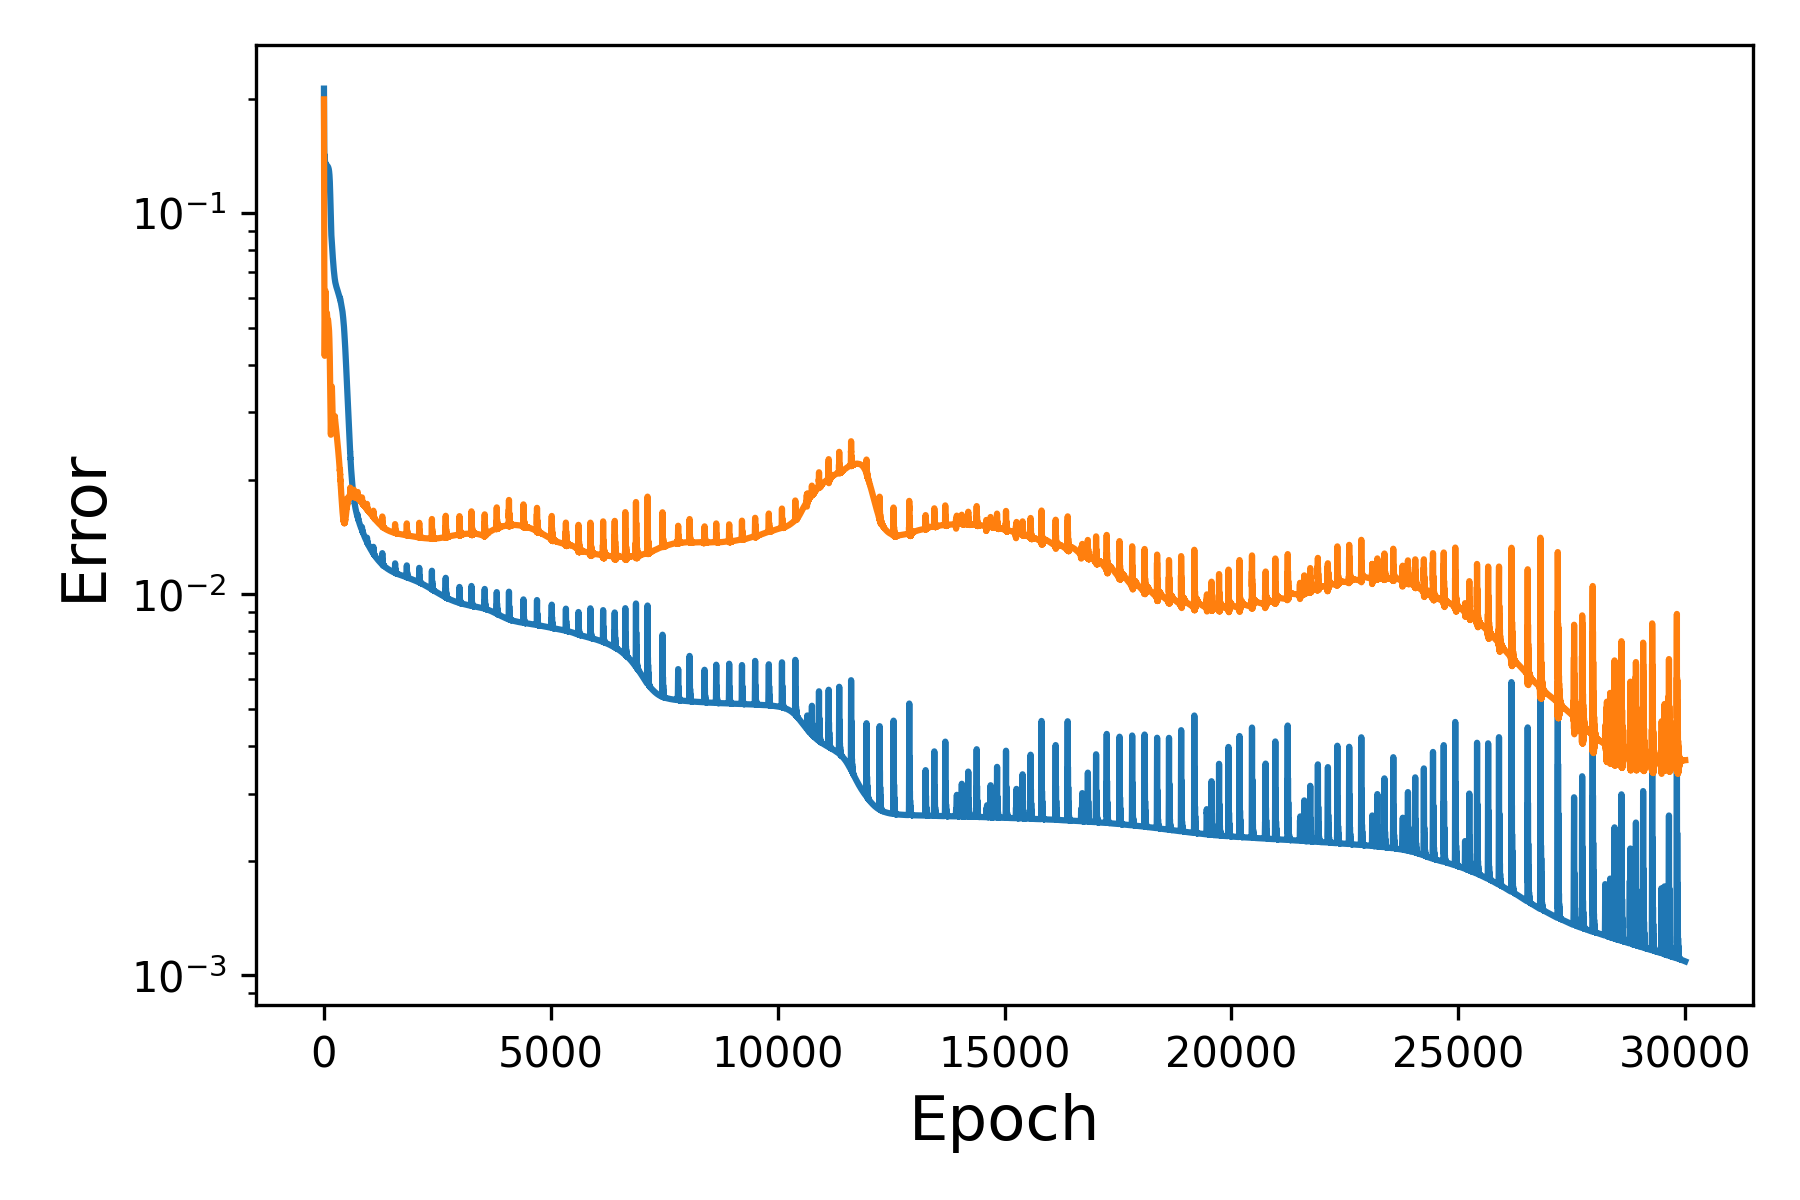
\includegraphics[width=1\linewidth]{./figs/sm_rep_loss_plot.png}  
		\caption{Standard learning rate.}
	\end{subfigure}
	\begin{subfigure}{.45\textwidth}
		\centering
		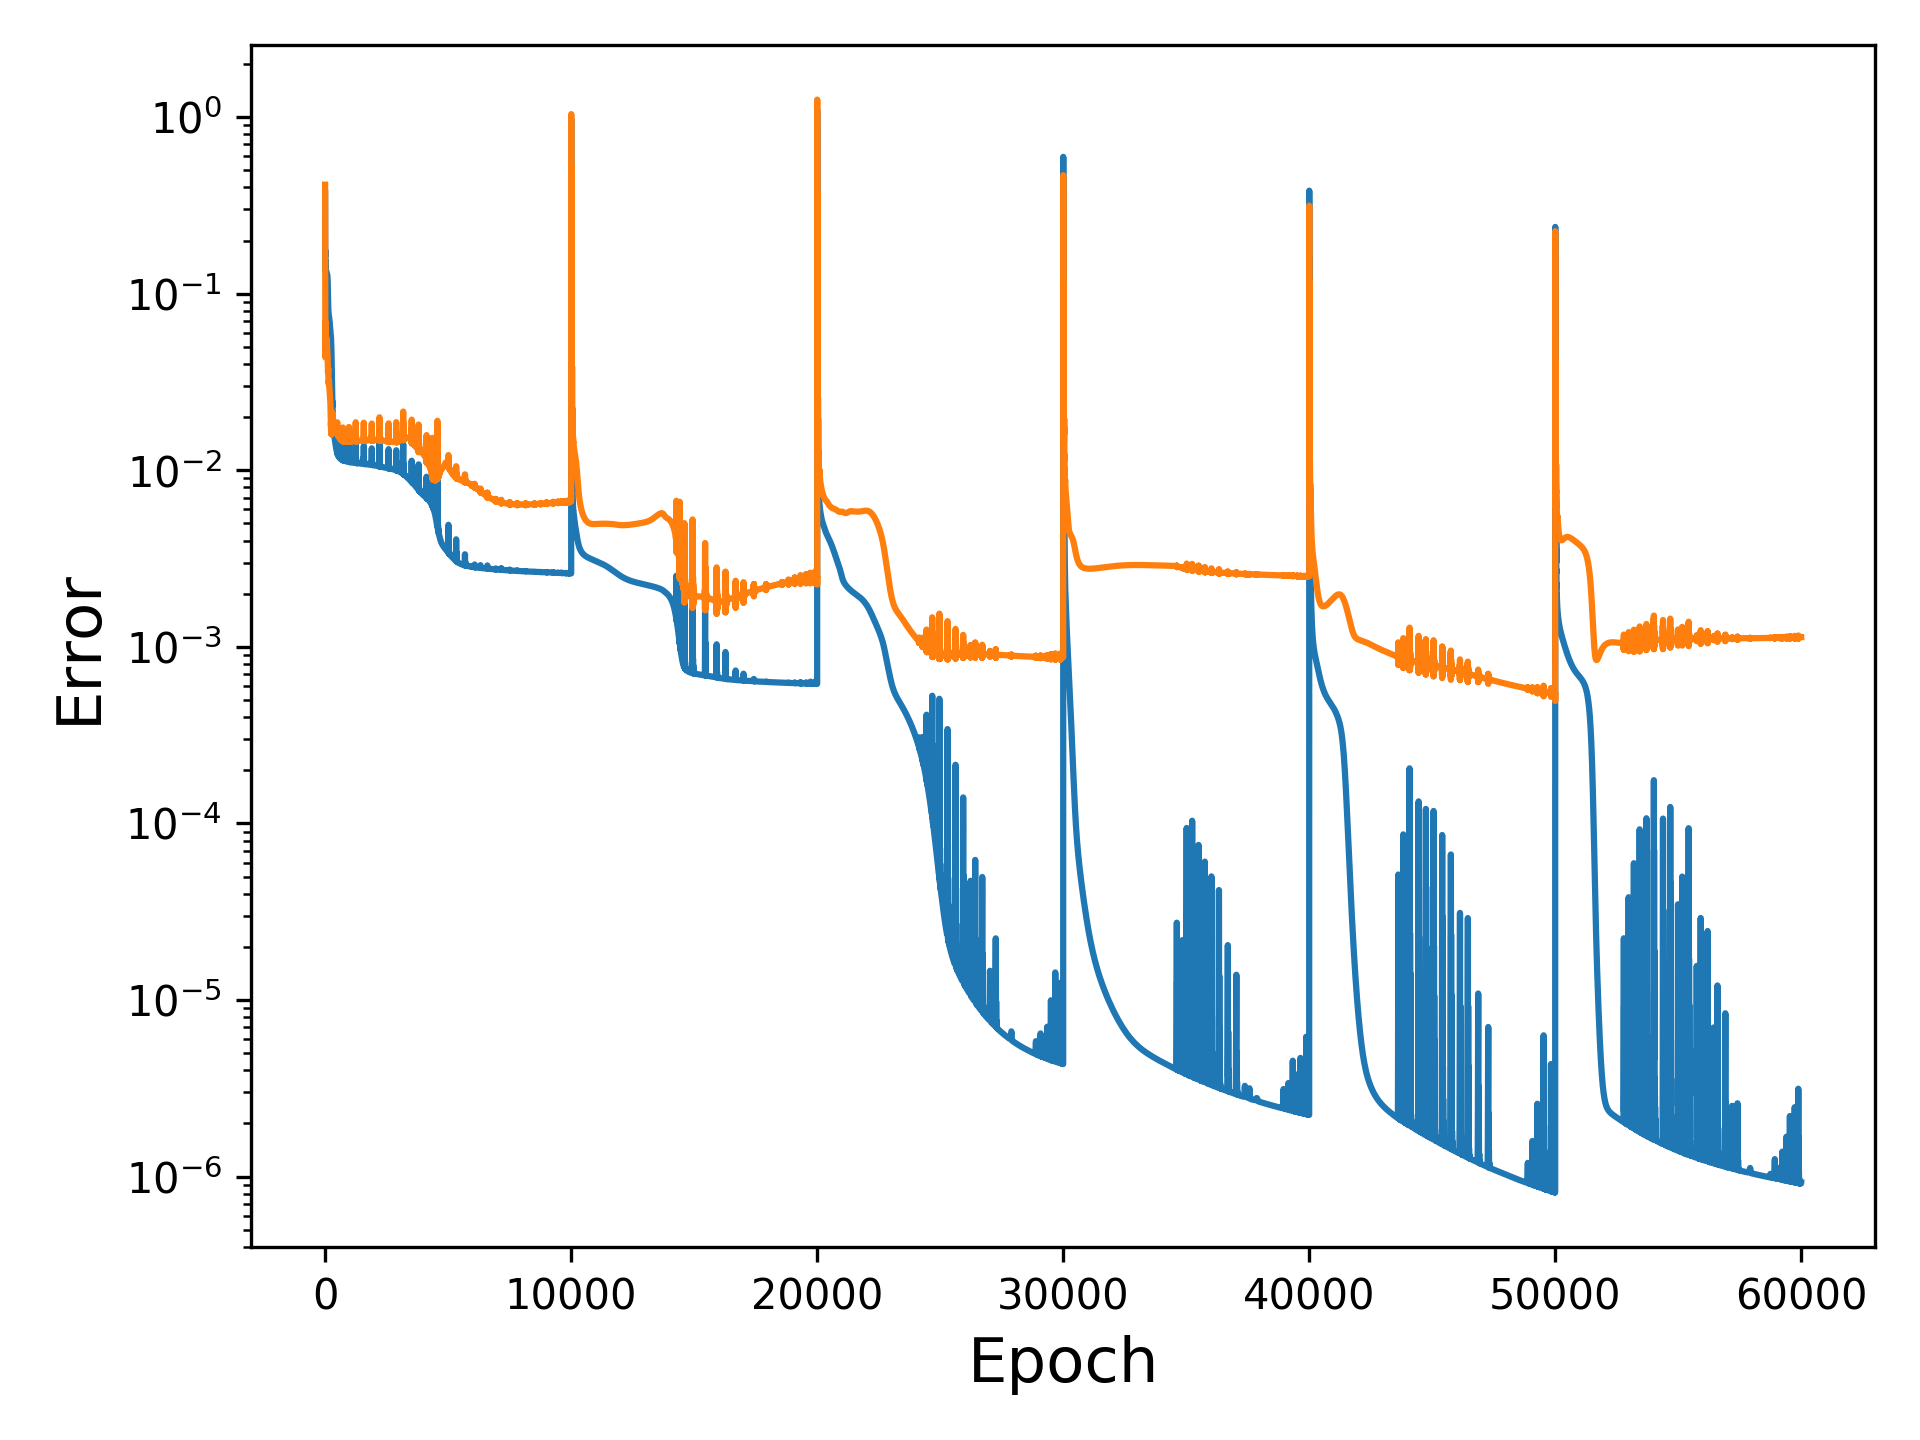
\includegraphics[width=1\linewidth]{./figs/snap_rep_loss_plot.png}  
		\caption{Cosine annealing.}
	\end{subfigure}
	\caption{Representative training/validation loss trajectories. Overfit begins after 60,000 epochs for this specific architecture.}
\end{figure}
\begin{figure}[H]
	\begin{subfigure}{.45\textwidth}
		\centering
		% include first image
		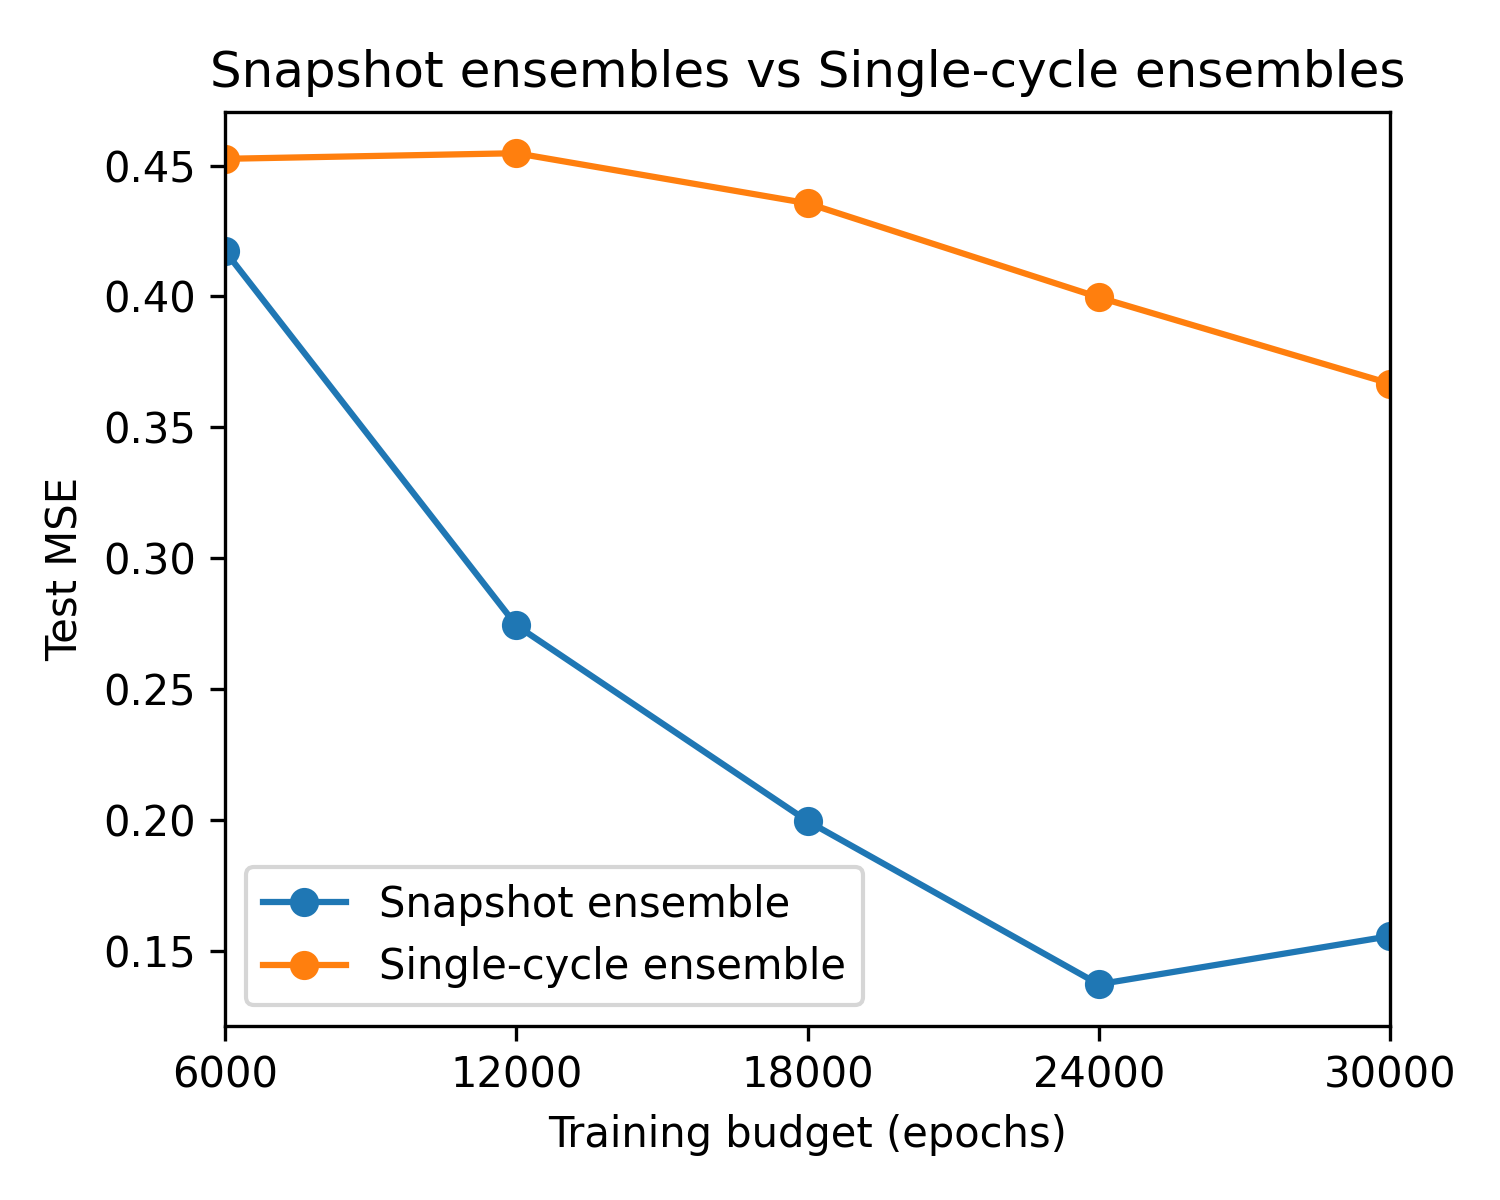
\includegraphics[width=1\linewidth]{./figs/vary_b.png}  
		\caption{Varying budget for fixed number of cycles and number of snapshots. Comparison with single-cycle ensemble (cosine annealing with random restarts). This is why we need \textit{warm restarts}.}
		\label{fig:sub-first}
	\end{subfigure}
	\begin{subfigure}{.45\textwidth}
		\centering
		% include second image
		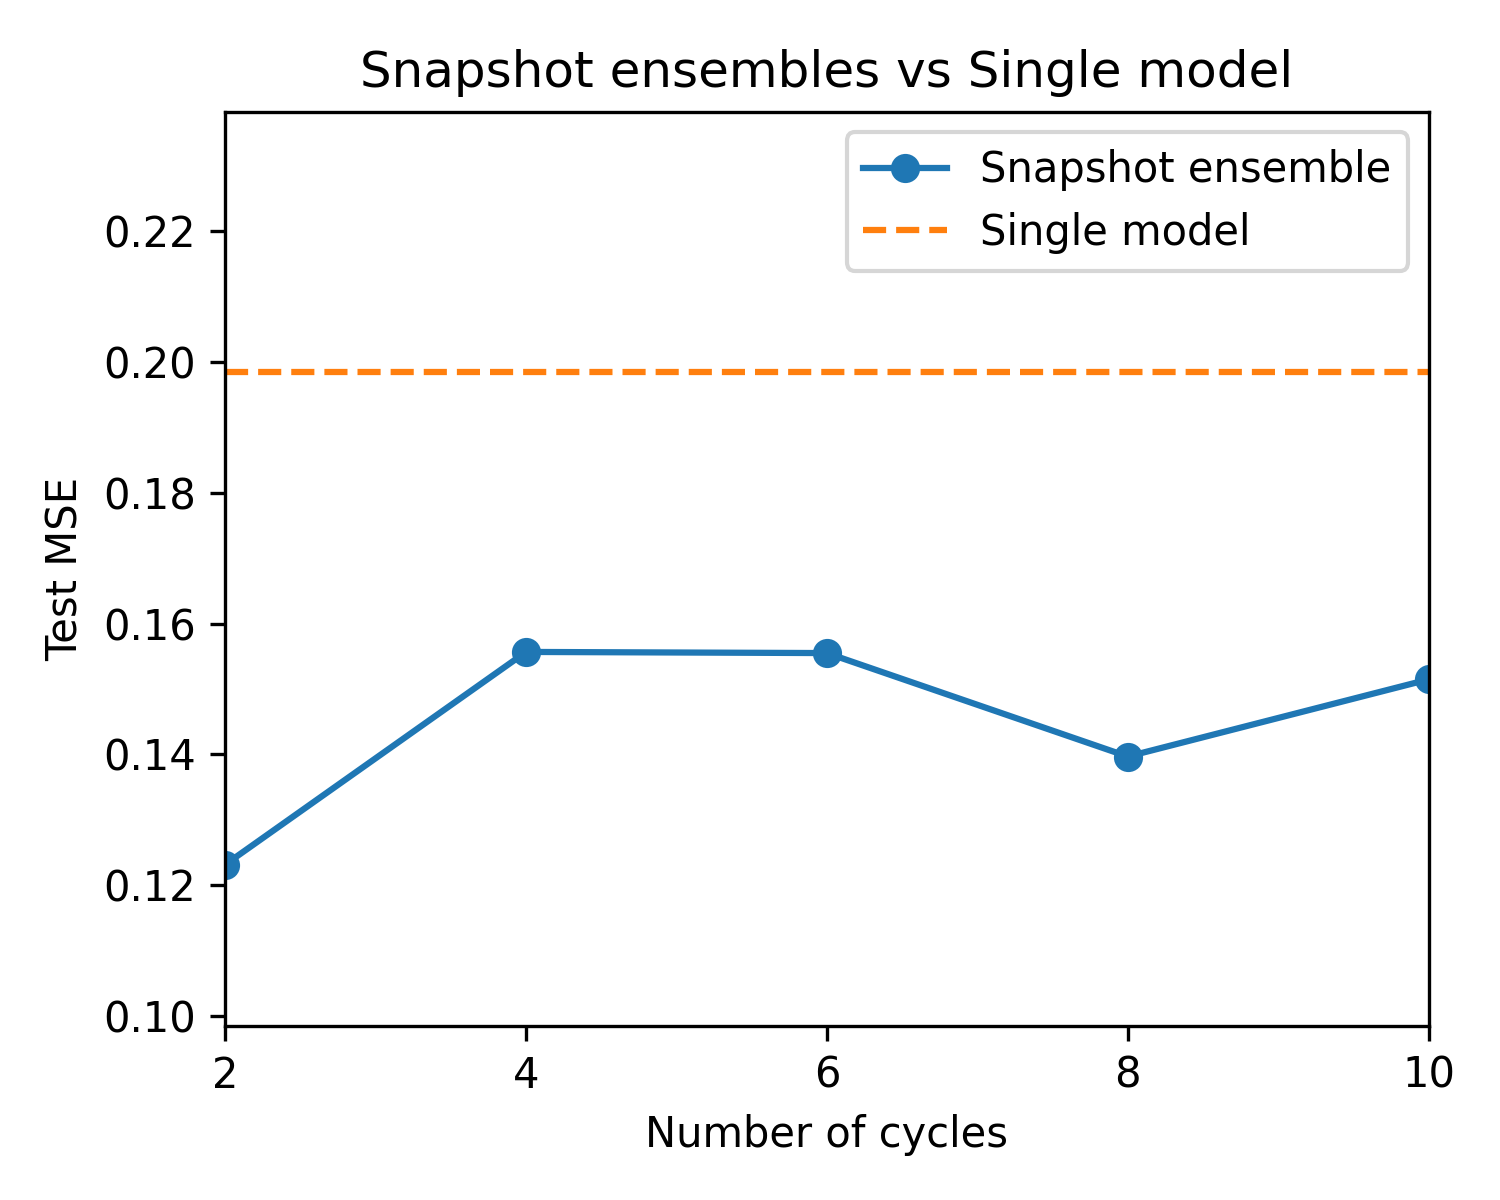
\includegraphics[width=1\linewidth]{./figs/vary_ac.png}  
		\caption{Varying number of cycles for fixed budget and number of snapshots (same as number of cycles).\newline\newline}
		\label{fig:sub-second}
	\end{subfigure}
	\begin{subfigure}{1\textwidth}
		\centering
		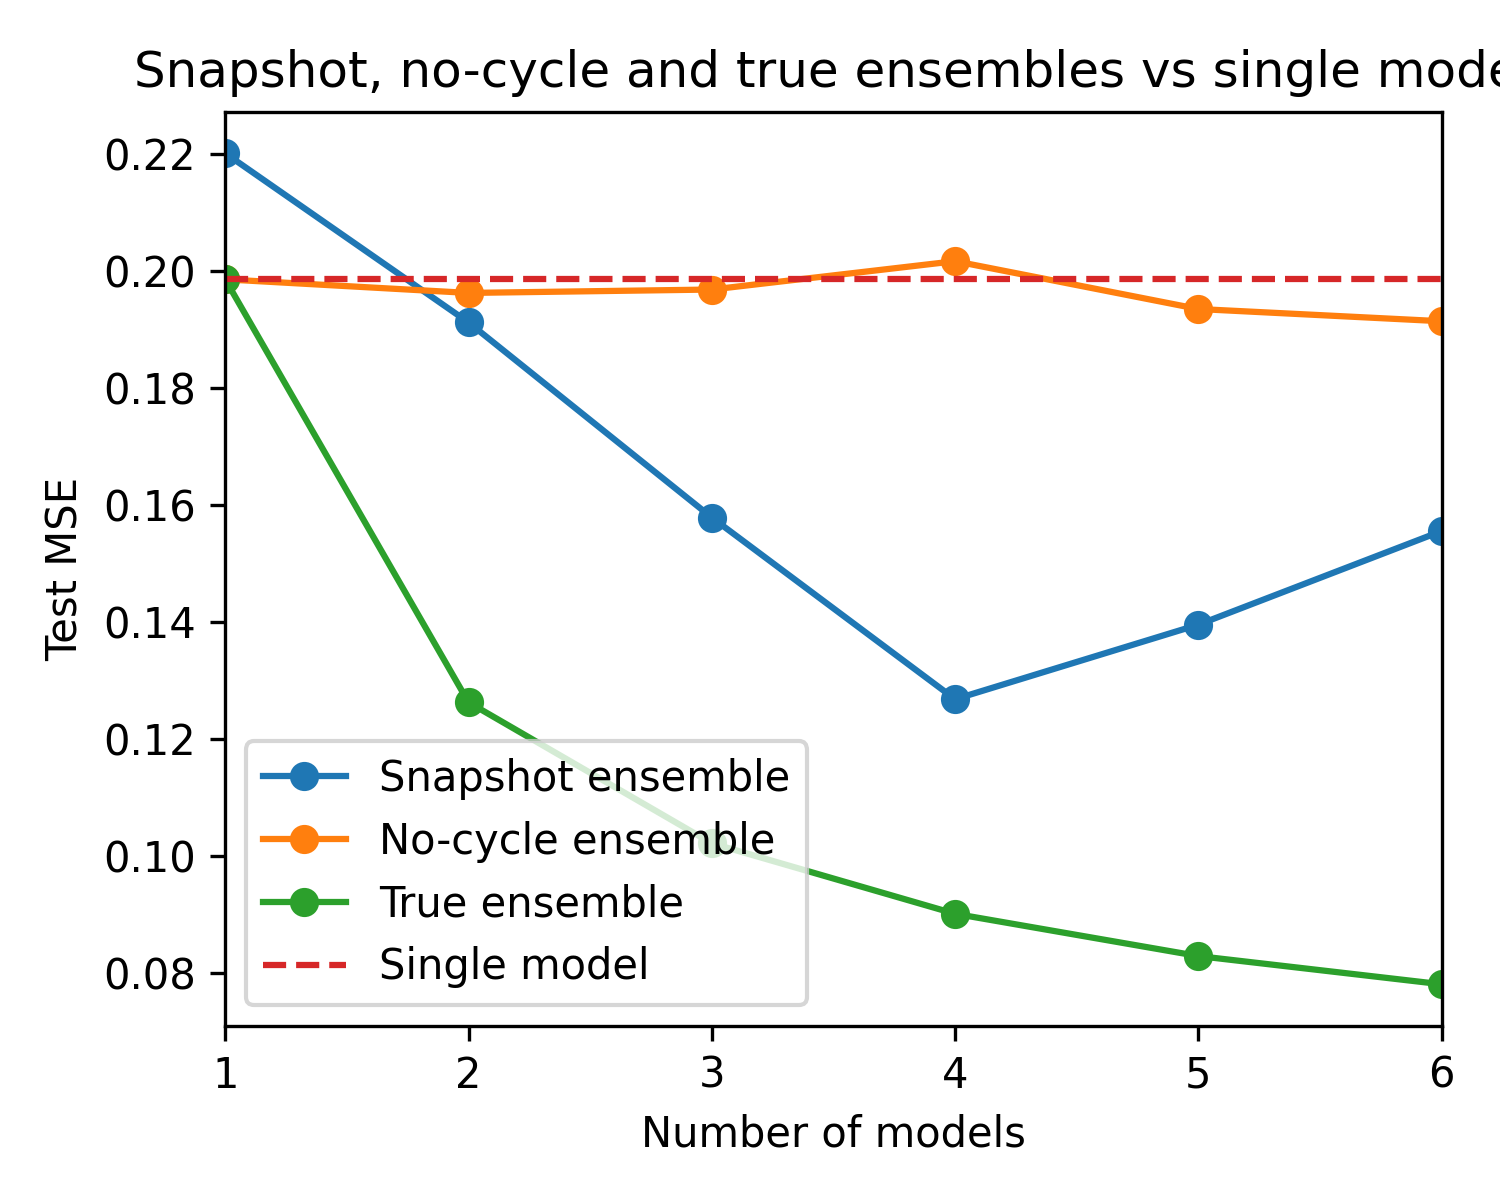
\includegraphics[width=.7\linewidth]{./figs/vary_snaps.png}  
		\caption{Snapshot ensemble (cosine annealing and varying number of snapshots), no-cycle ensemble (standard lr and varying number of snapshots), true ensemble (varying number of trajectories), and super ensemble (varying number of trajectories and fixed number of snapshots). Budget and number of cycles is fixed for all cases.}
		\label{fig:sub-second}
	\end{subfigure}
	\caption{Relative $\ell_2$ test error. Comparisons between single models, snapshot ensembles, no-cycle ensembles (standard lr), single-cycle ensembles (cosine annealing with no warm restarts), and true ensembles.}
	\label{fig:fig}
\end{figure}

\begin{figure}[H]
	\centering
	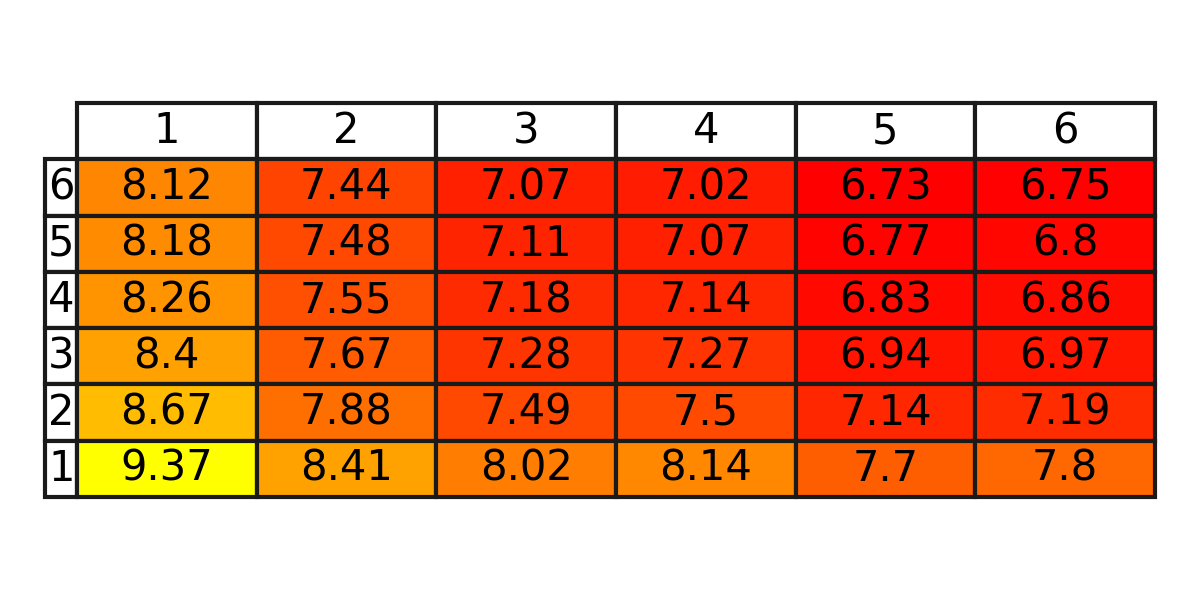
\includegraphics[width=0.6\linewidth]{./figs/kmn_plot.png}  
	\caption{Super ensembles: Relative $\%$ $\ell_2$ test error for varying number of trajectories (rows) and number of snapshots in a trajectory (columns).}
	\label{fig:sub-first}
\end{figure}

\begin{figure}[H]
	\centering
	\begin{subfigure}{.45\textwidth}
		\centering
		% include first image
		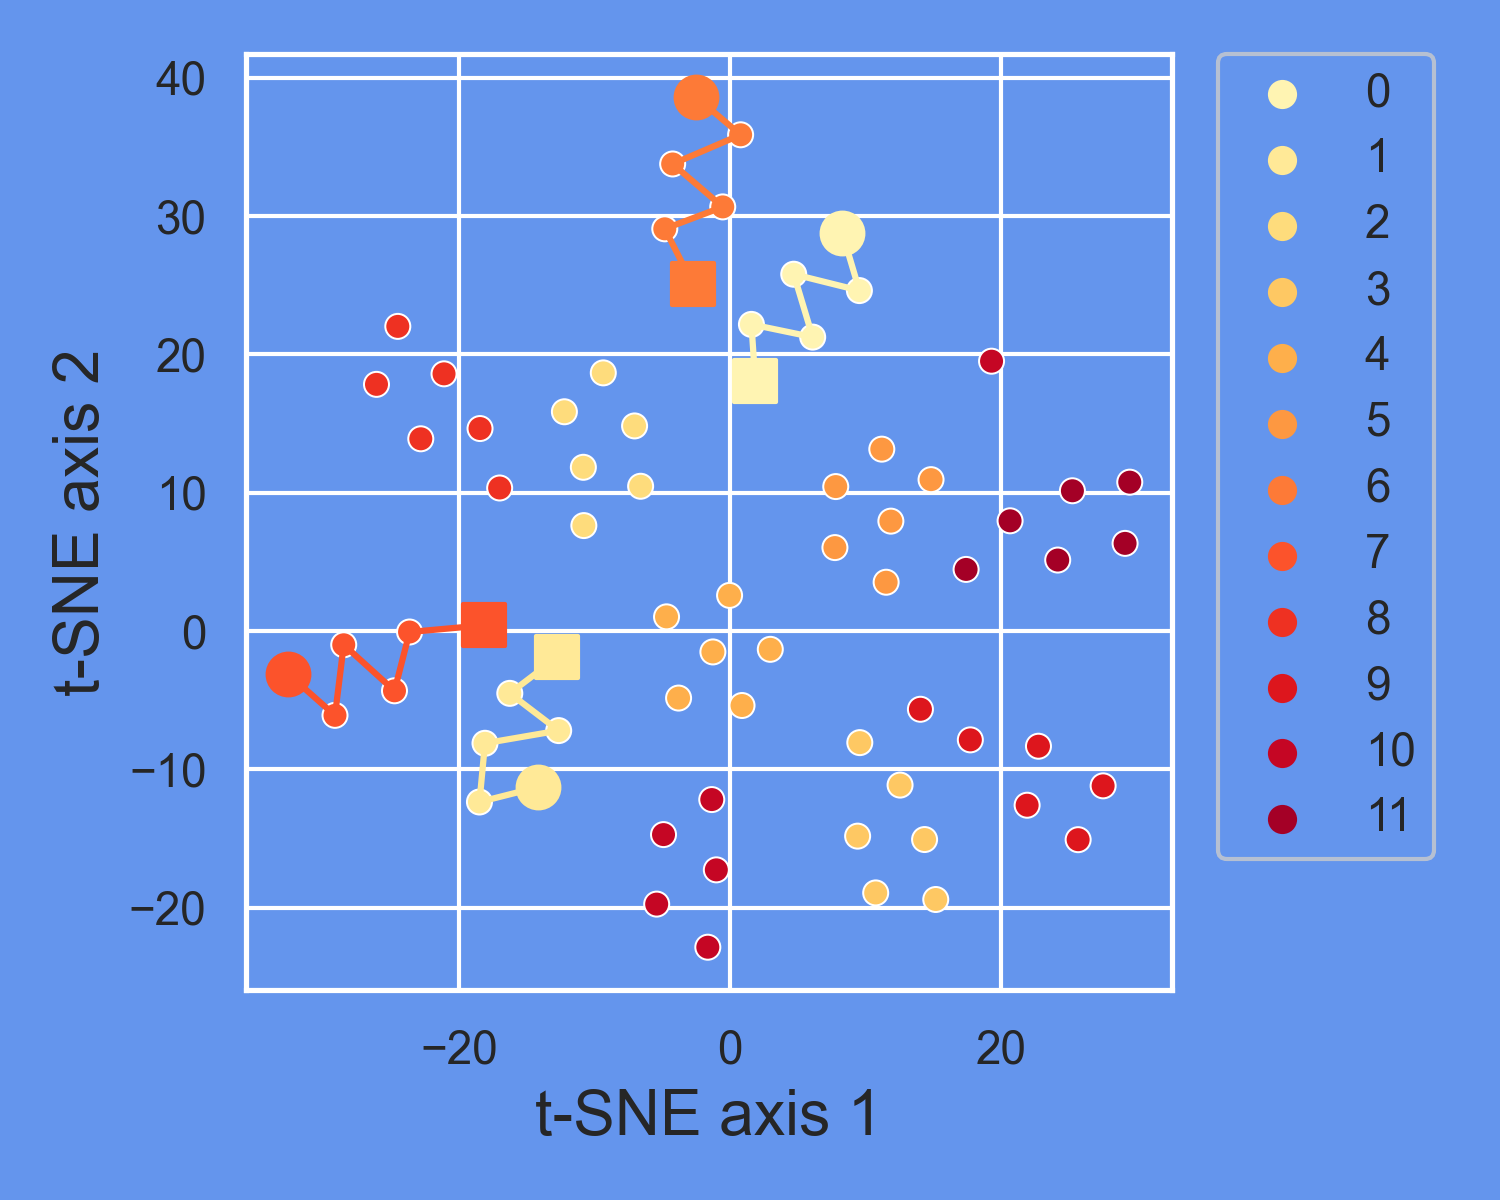
\includegraphics[width=.9\linewidth]{./figs/params_tSNE_0.png}  
		\caption{2 trajectories with standard learning rate (light colors) and 2 with cosine annealing (dark colors).}
		\label{fig:sub-first}
	\end{subfigure}
	\begin{subfigure}{.45\textwidth}
		\centering
		% include second image
		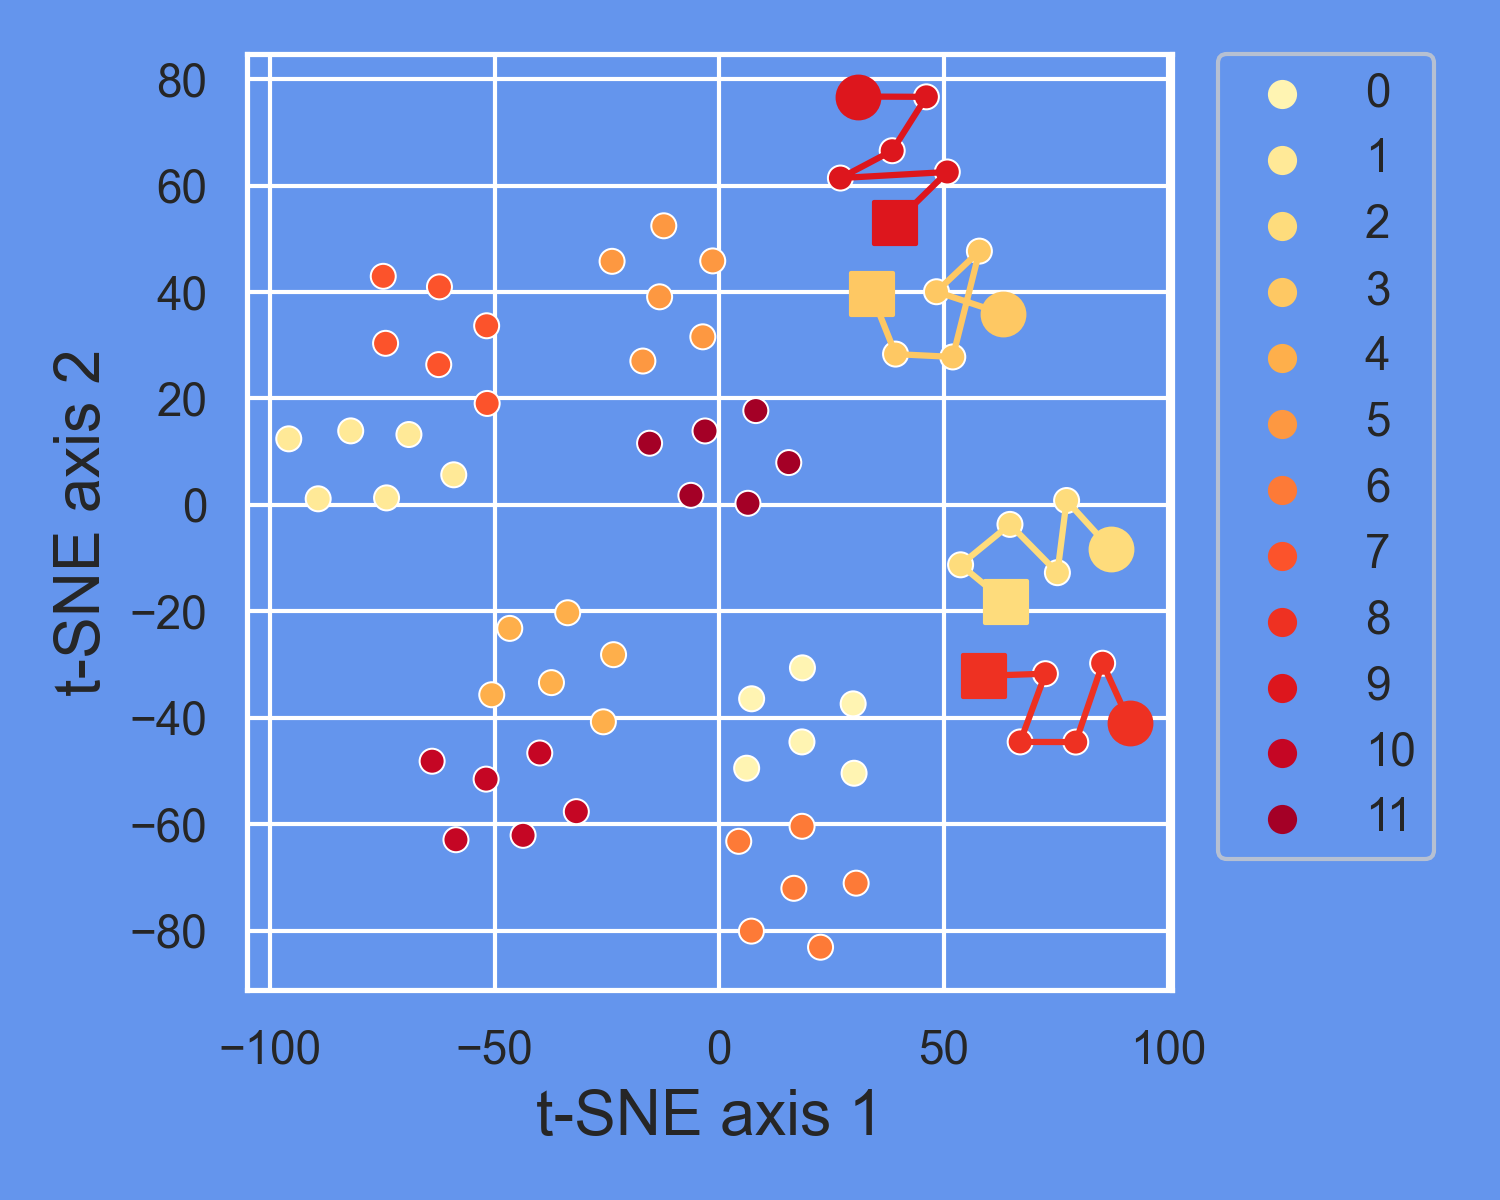
\includegraphics[width=.9\linewidth]{./figs/params_tSNE_1.png}  
		\caption{2 trajectories with standard learning rate (light colors) and 2 with cosine annealing (dark colors).}
		\label{fig:sub-second}
	\end{subfigure}
	\begin{subfigure}{.45\textwidth}
		\centering
		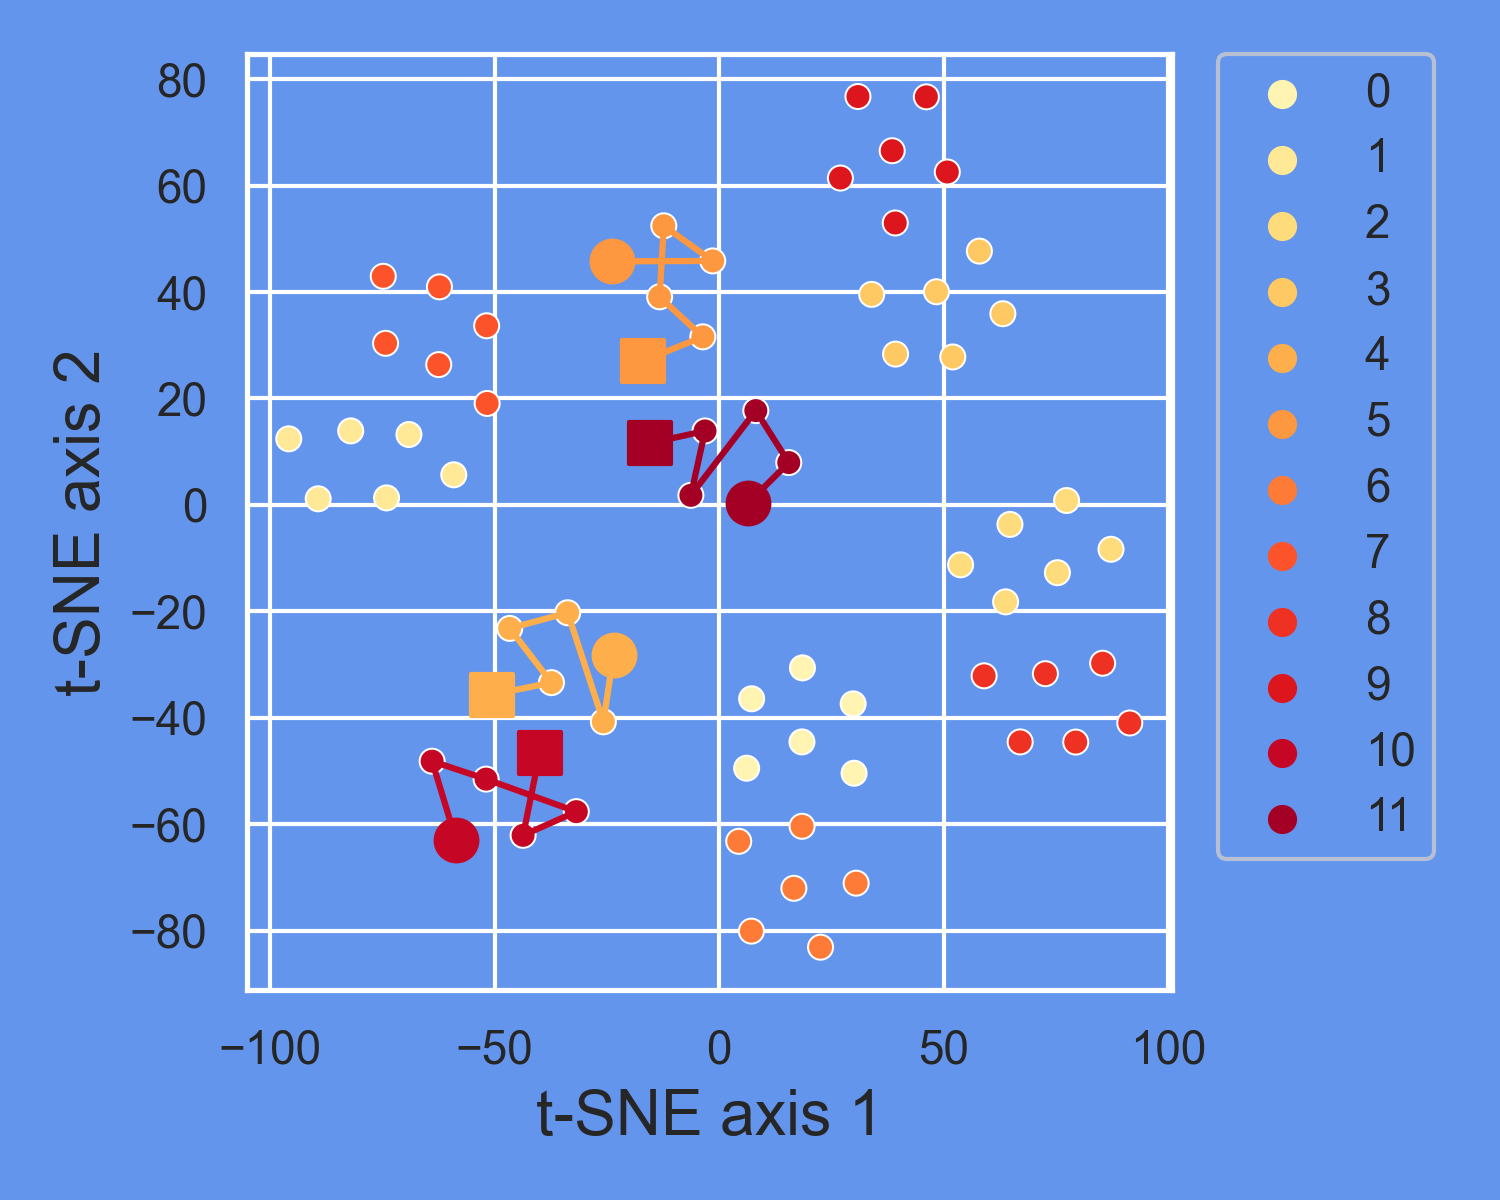
\includegraphics[width=.9\linewidth]{./figs/params_tSNE_2.png}  
		\caption{2 trajectories with standard learning rate (light colors) and 2 with cosine annealing (dark colors).}
		\label{fig:sub-second}
	\end{subfigure}
	\caption{t-SNE of parameters from different trajectories for both standard learning rate and cosine annealing. Large circles represent final parameters, small circles earlier snapshots and squares the earliest considered snapshots (not necessarily the initializations). Lighter colors represent standard learning rate and darker colors cosine annealing.}
	\label{fig:fig}
\end{figure}

\begin{figure}[H]
	\centering
	\begin{subfigure}{.45\textwidth}
		\centering
		% include first image
		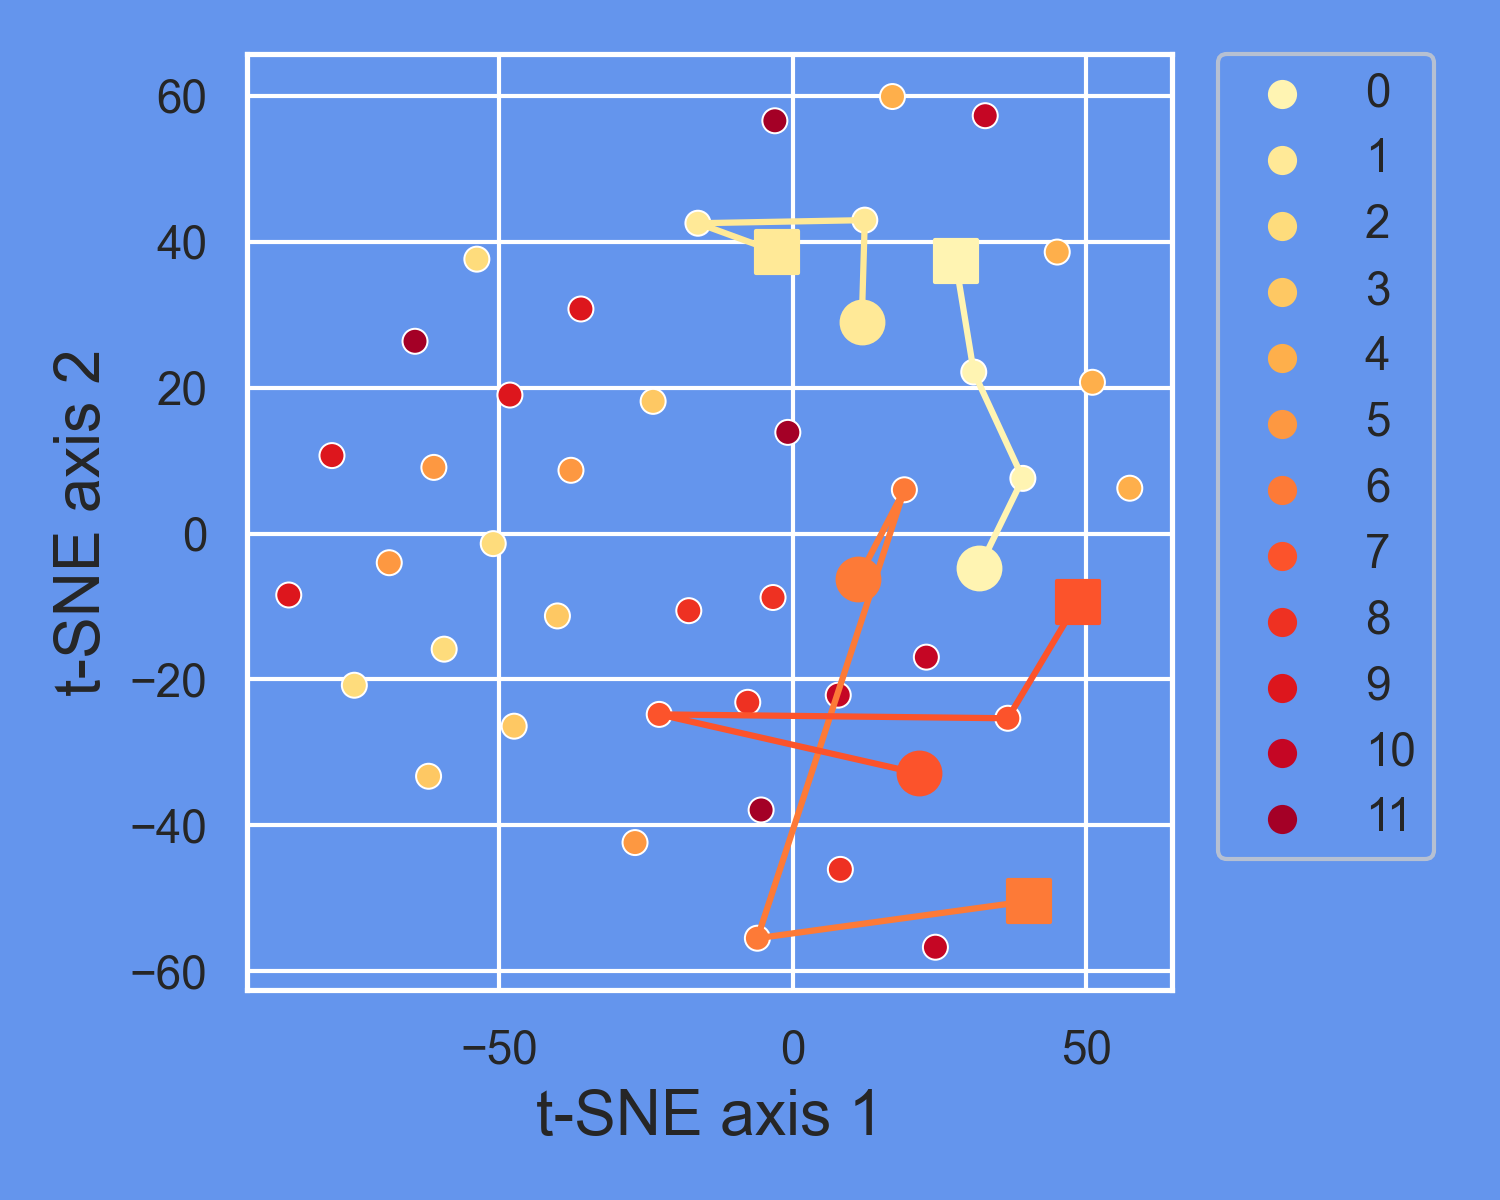
\includegraphics[width=.9\linewidth]{./figs/preds_tSNE_0.png}  
		\caption{2 trajectories with standard learning rate (light colors) and 2 with cosine annealing (dark colors).}
		\label{fig:sub-first}
	\end{subfigure}
	\begin{subfigure}{.45\textwidth}
		\centering
		% include second image
		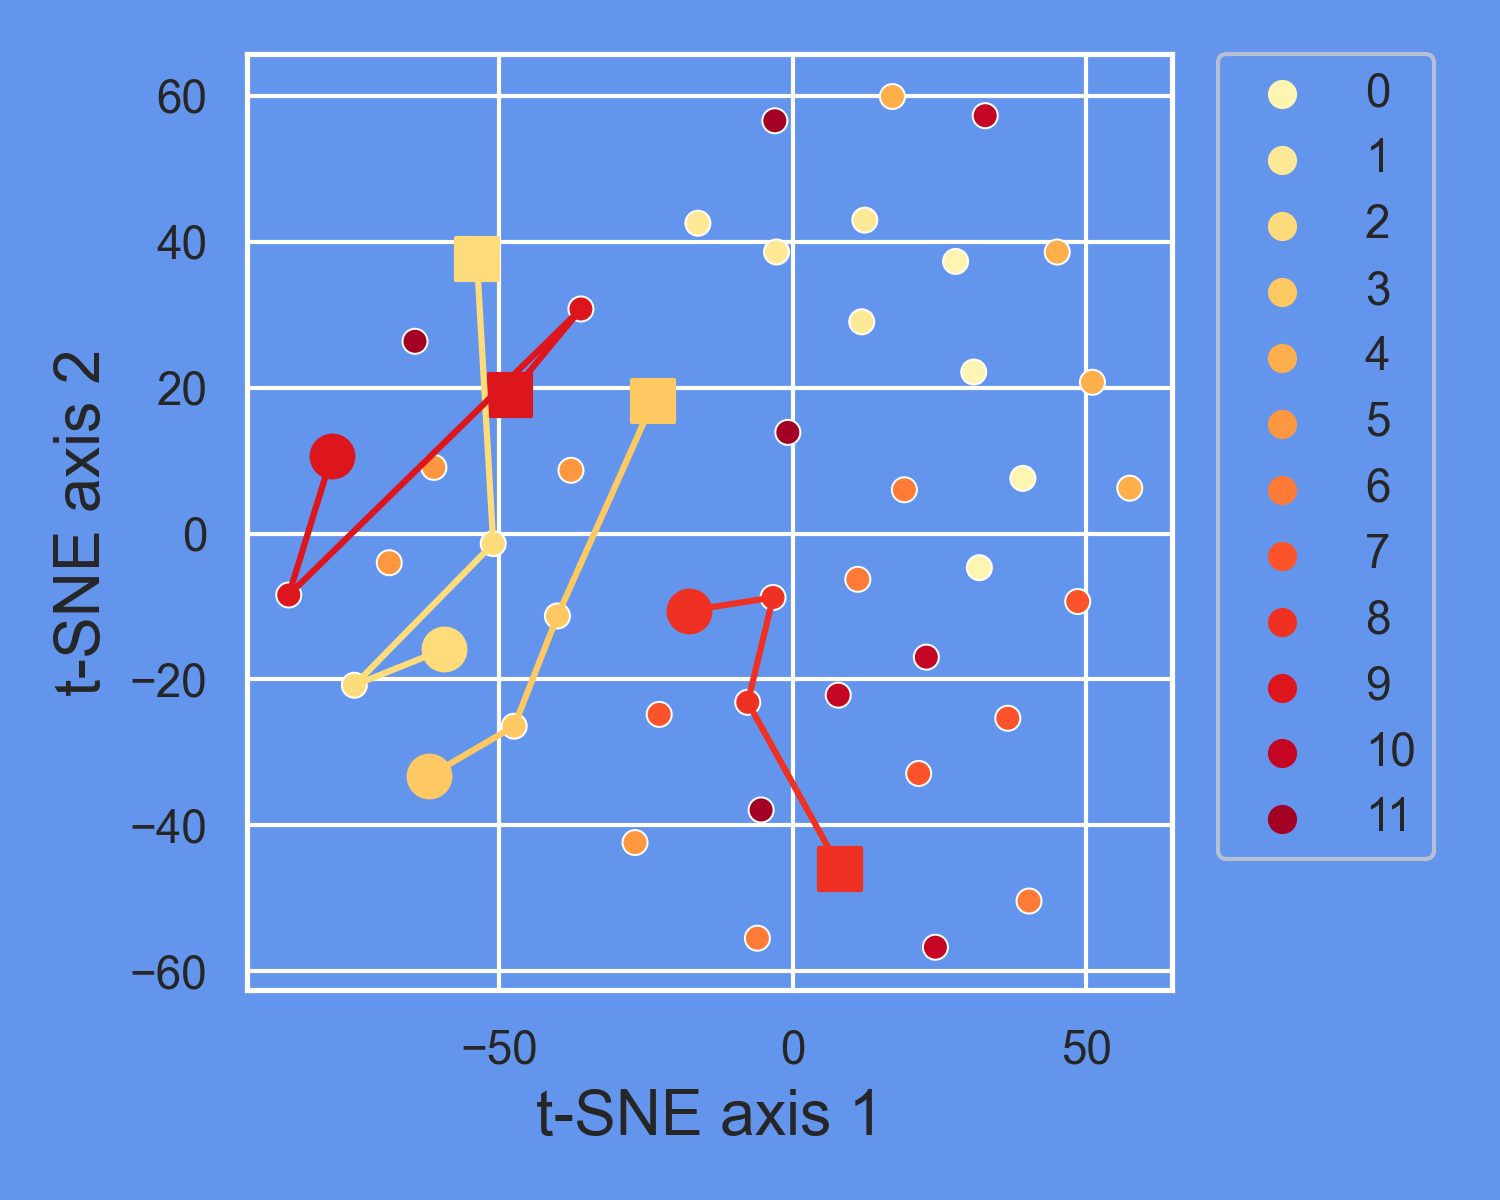
\includegraphics[width=.9\linewidth]{./figs/preds_tSNE_1.png}  
		\caption{2 trajectories with standard learning rate (light colors) and 2 with cosine annealing (dark colors).}
		\label{fig:sub-second}
	\end{subfigure}	
	\begin{subfigure}{.45\textwidth}
		\centering
		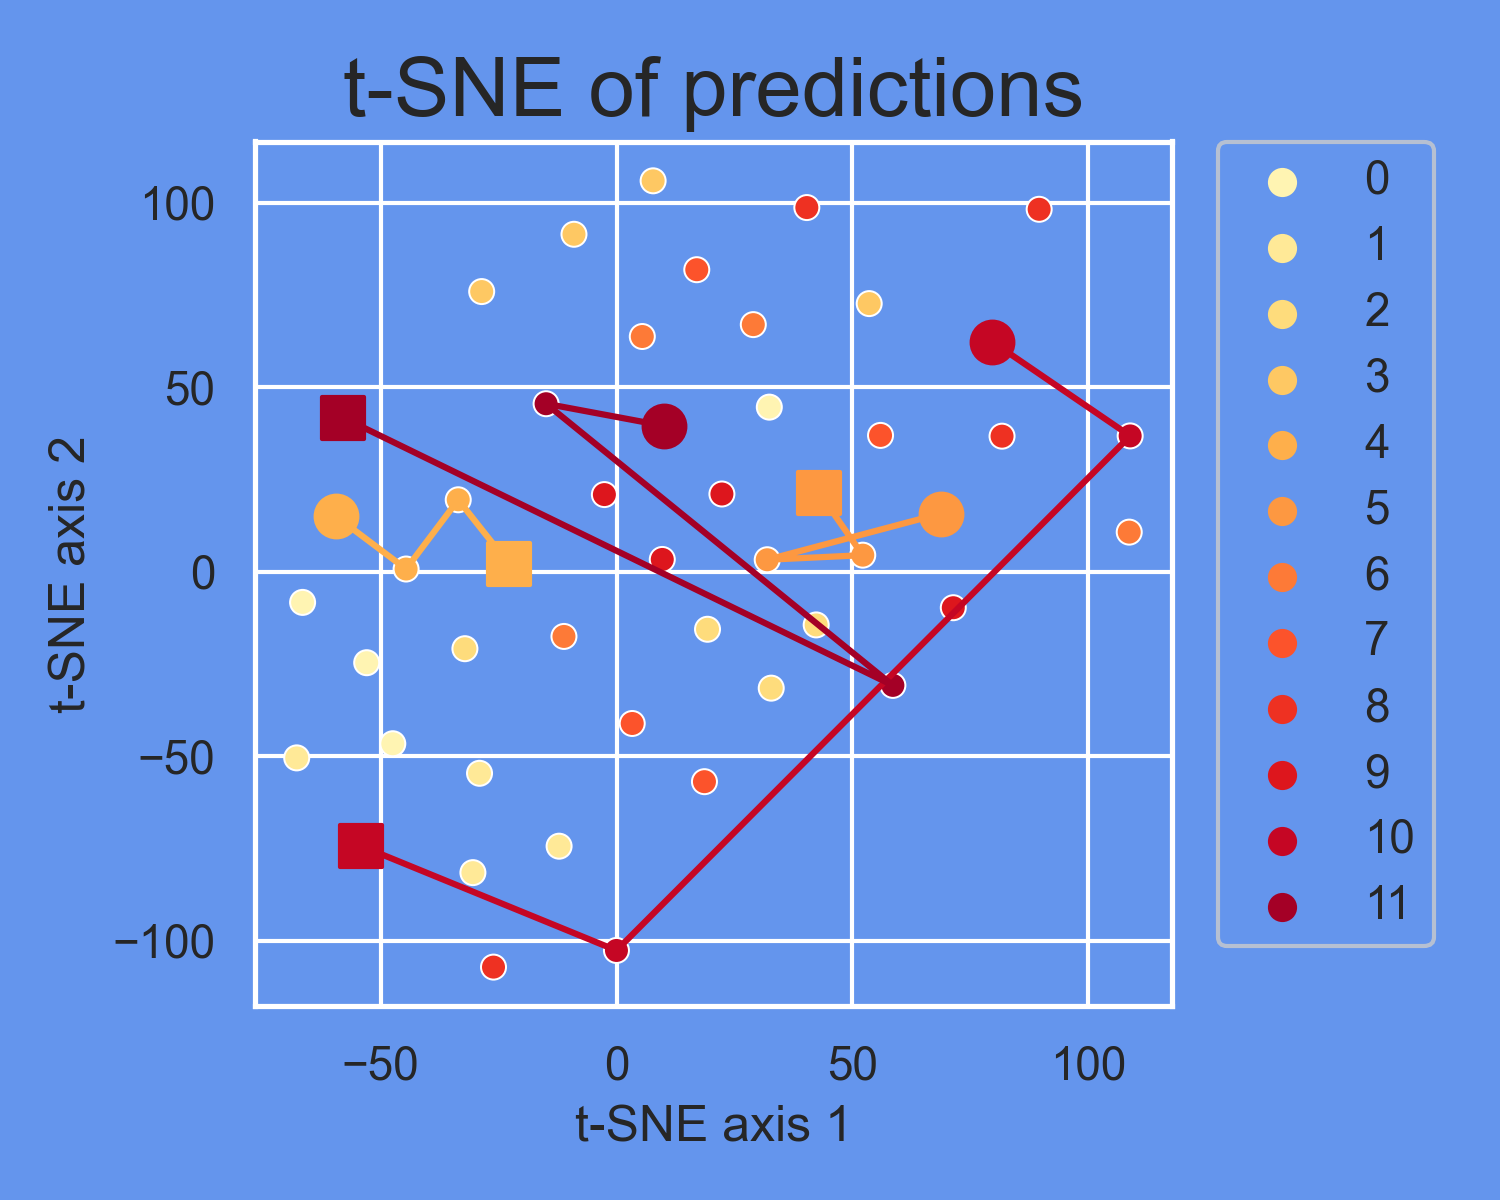
\includegraphics[width=.9\linewidth]{./figs/preds_tSNE_2.png}  
		\caption{2 trajectories with standard learning rate (light colors) and 2 with cosine annealing (dark colors).}
		\label{fig:sub-second}
	\end{subfigure}
	\caption{t-SNE of predicted functions from different trajectories for both standard learning rate and cosine annealing. Large circles represent predictions corresponding to final parameters, small circles to earlier snapshots and squares to the earliest considered snapshots (not necessarily the initializations). Lighter colors represent standard learning rate and darker colors cosine annealing.}
	\label{fig:fig}
\end{figure}

\begin{figure}[H]
	\centering
	\begin{subfigure}{1\textwidth}
		\centering
		% include first image
		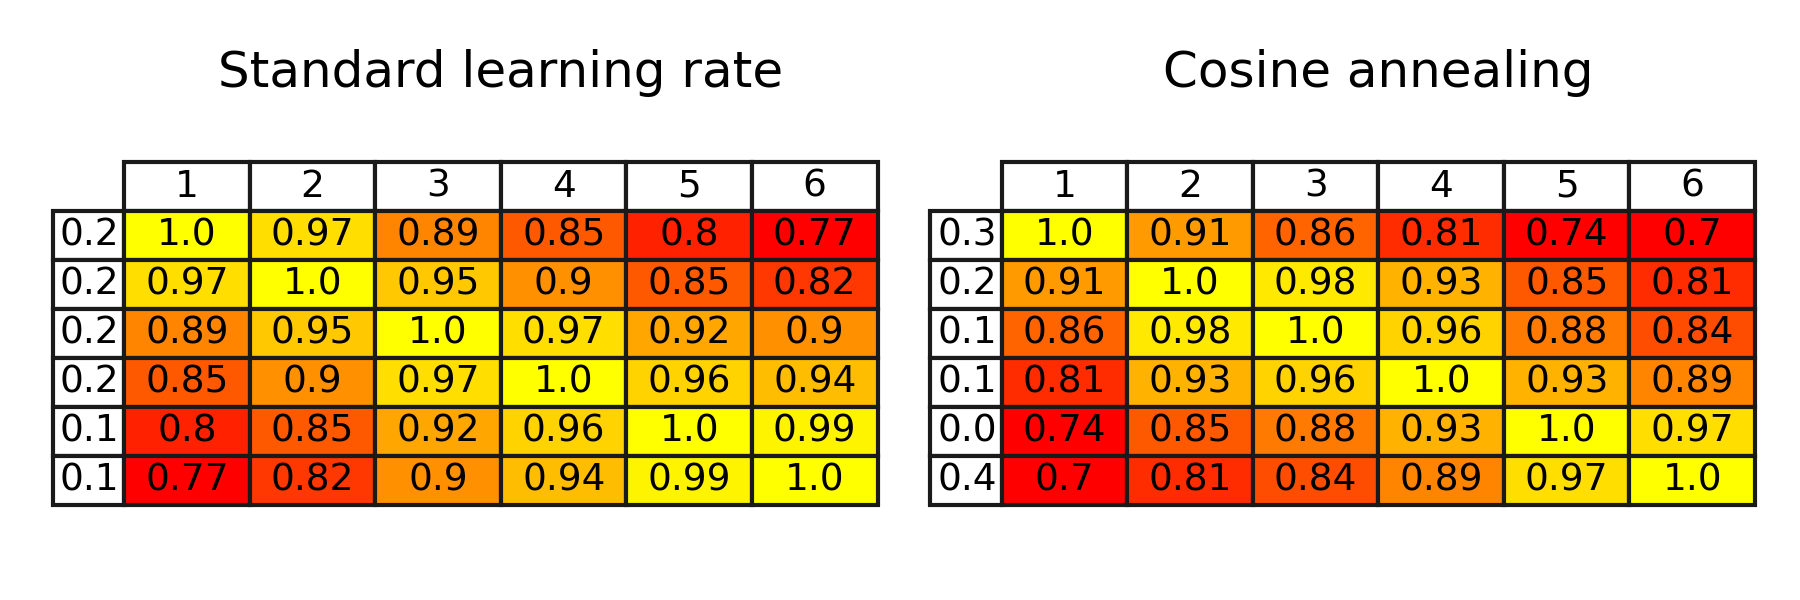
\includegraphics[width=1\linewidth]{./figs/params_cosine_similarities.png}  
		\caption{Cosine similarity ($\%$) of parameters corresponding to different snapshots. Far-left column shows the associated relative $\ell_2$ test error.}
		\label{fig:sub-first}
	\end{subfigure}
	\begin{subfigure}{1\textwidth}
		\centering
		% include second image
		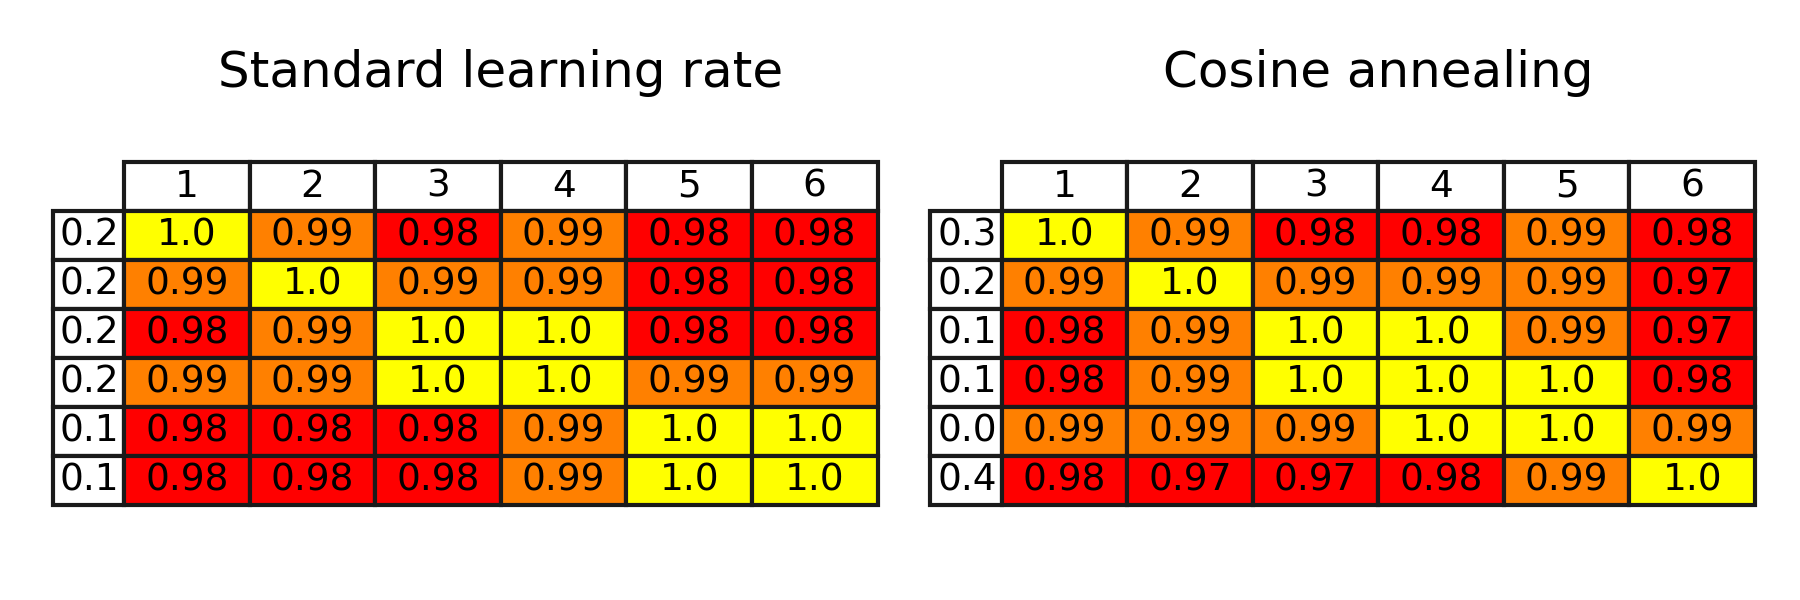
\includegraphics[width=1\linewidth]{./figs/preds_cosine_similarities.png}  
		\caption{Cosine similarity ($\%$) of predicted functions corresponding to different snapshots. Far-left column shows the associated relative $\ell_2$ test error.}
		\label{fig:sub-second}
	\end{subfigure}	
\end{figure}

\begin{figure}[H]
	\centering
	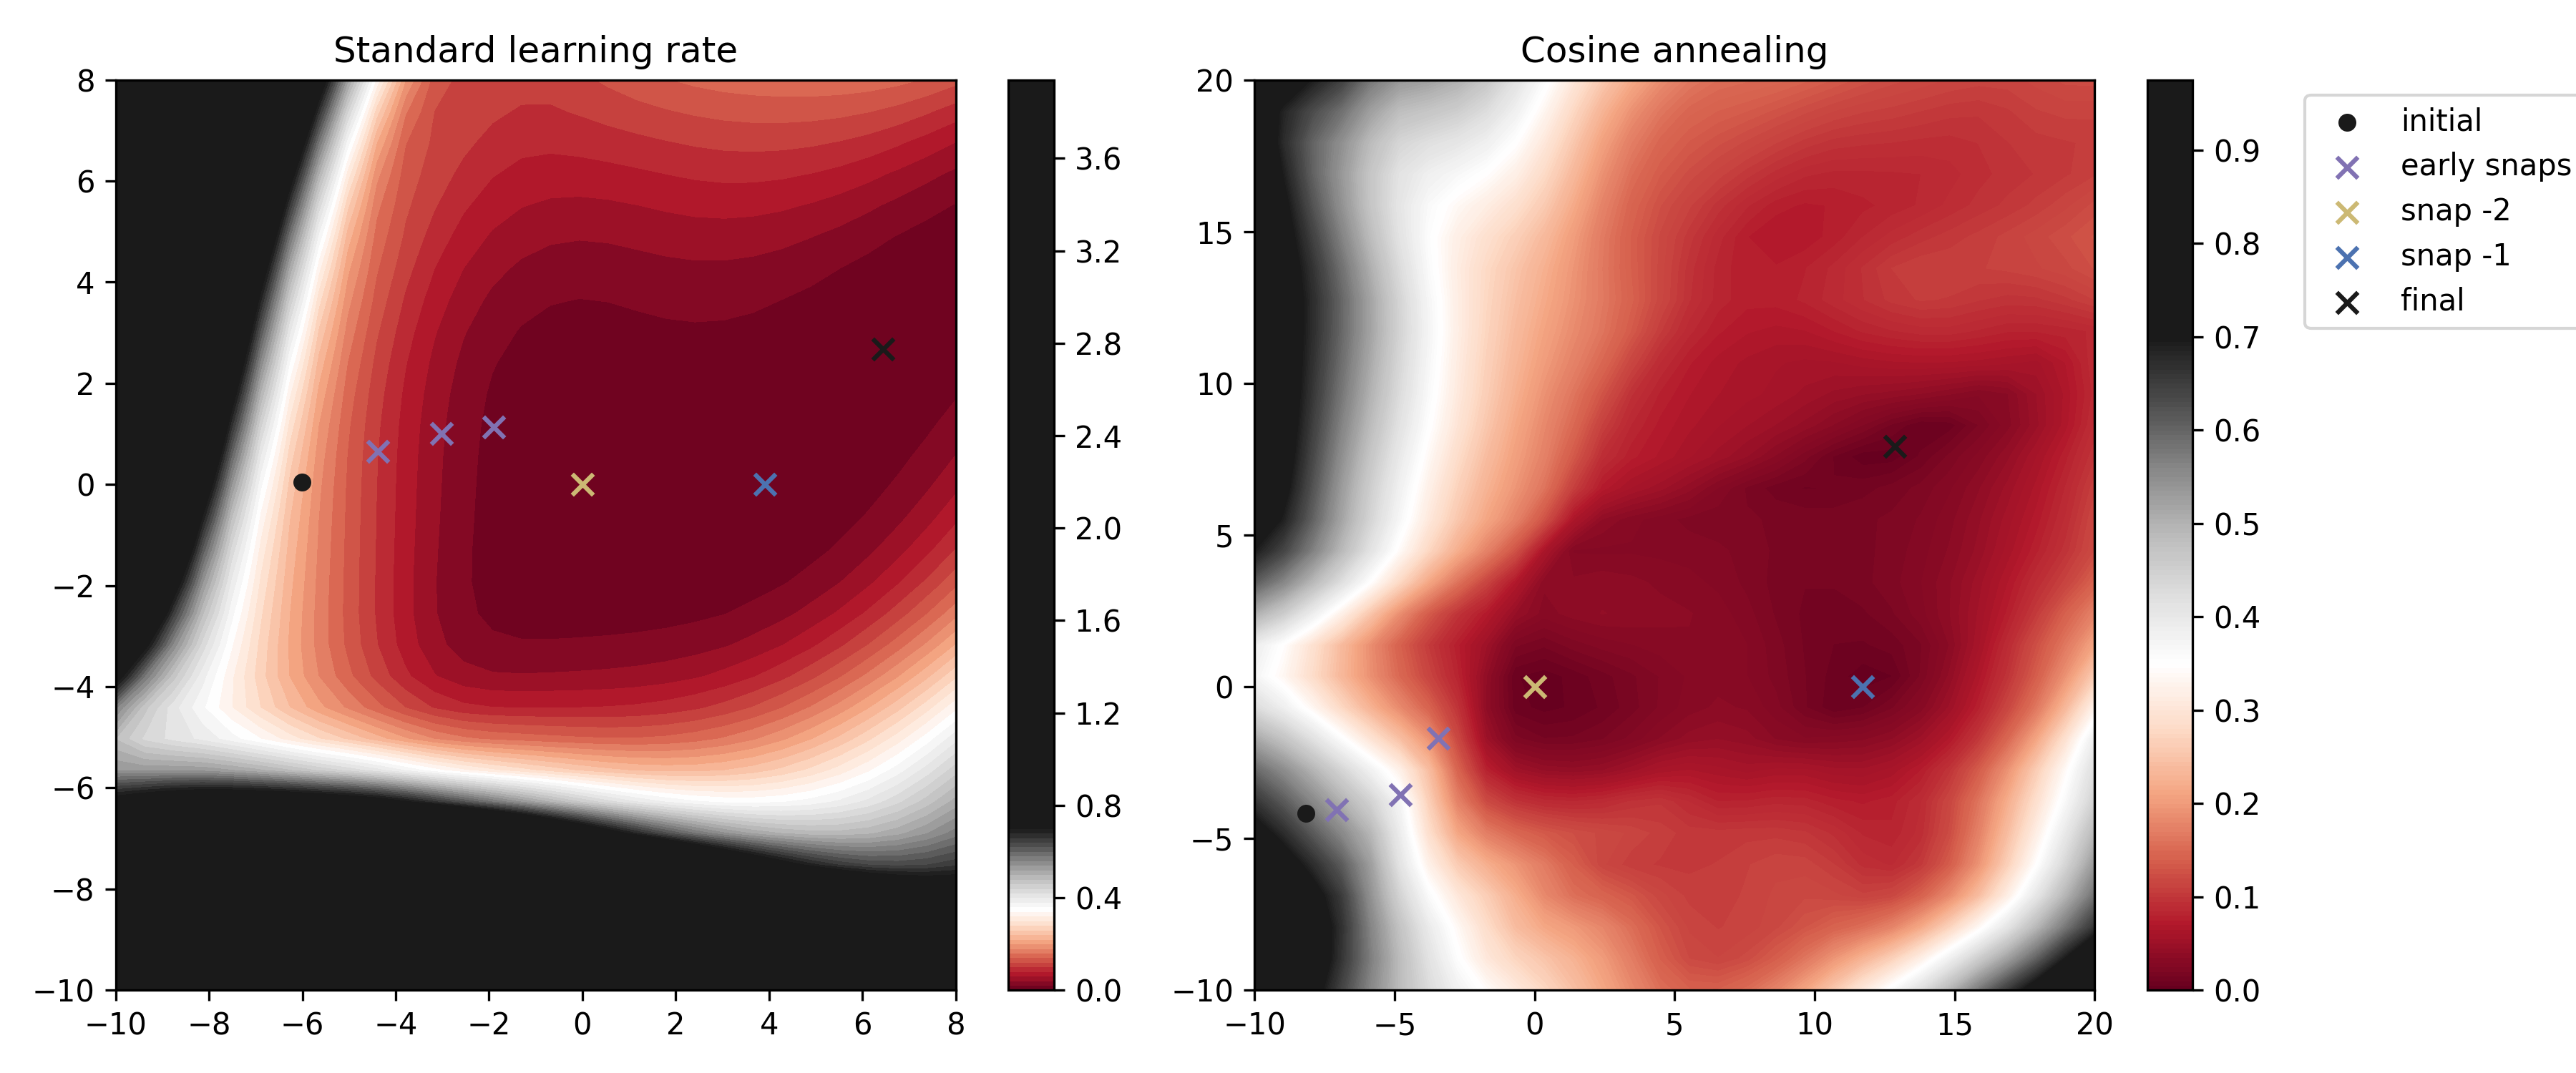
\includegraphics[width=1\linewidth]{./figs/planes.png}  
	\caption{Training loss on the plane defined by the last 3 snapshots of one trajectory. Earlier snapshots and initial parameters are projected on the plane.}
	\label{}
\end{figure}

\begin{figure}[H]
	\centering
	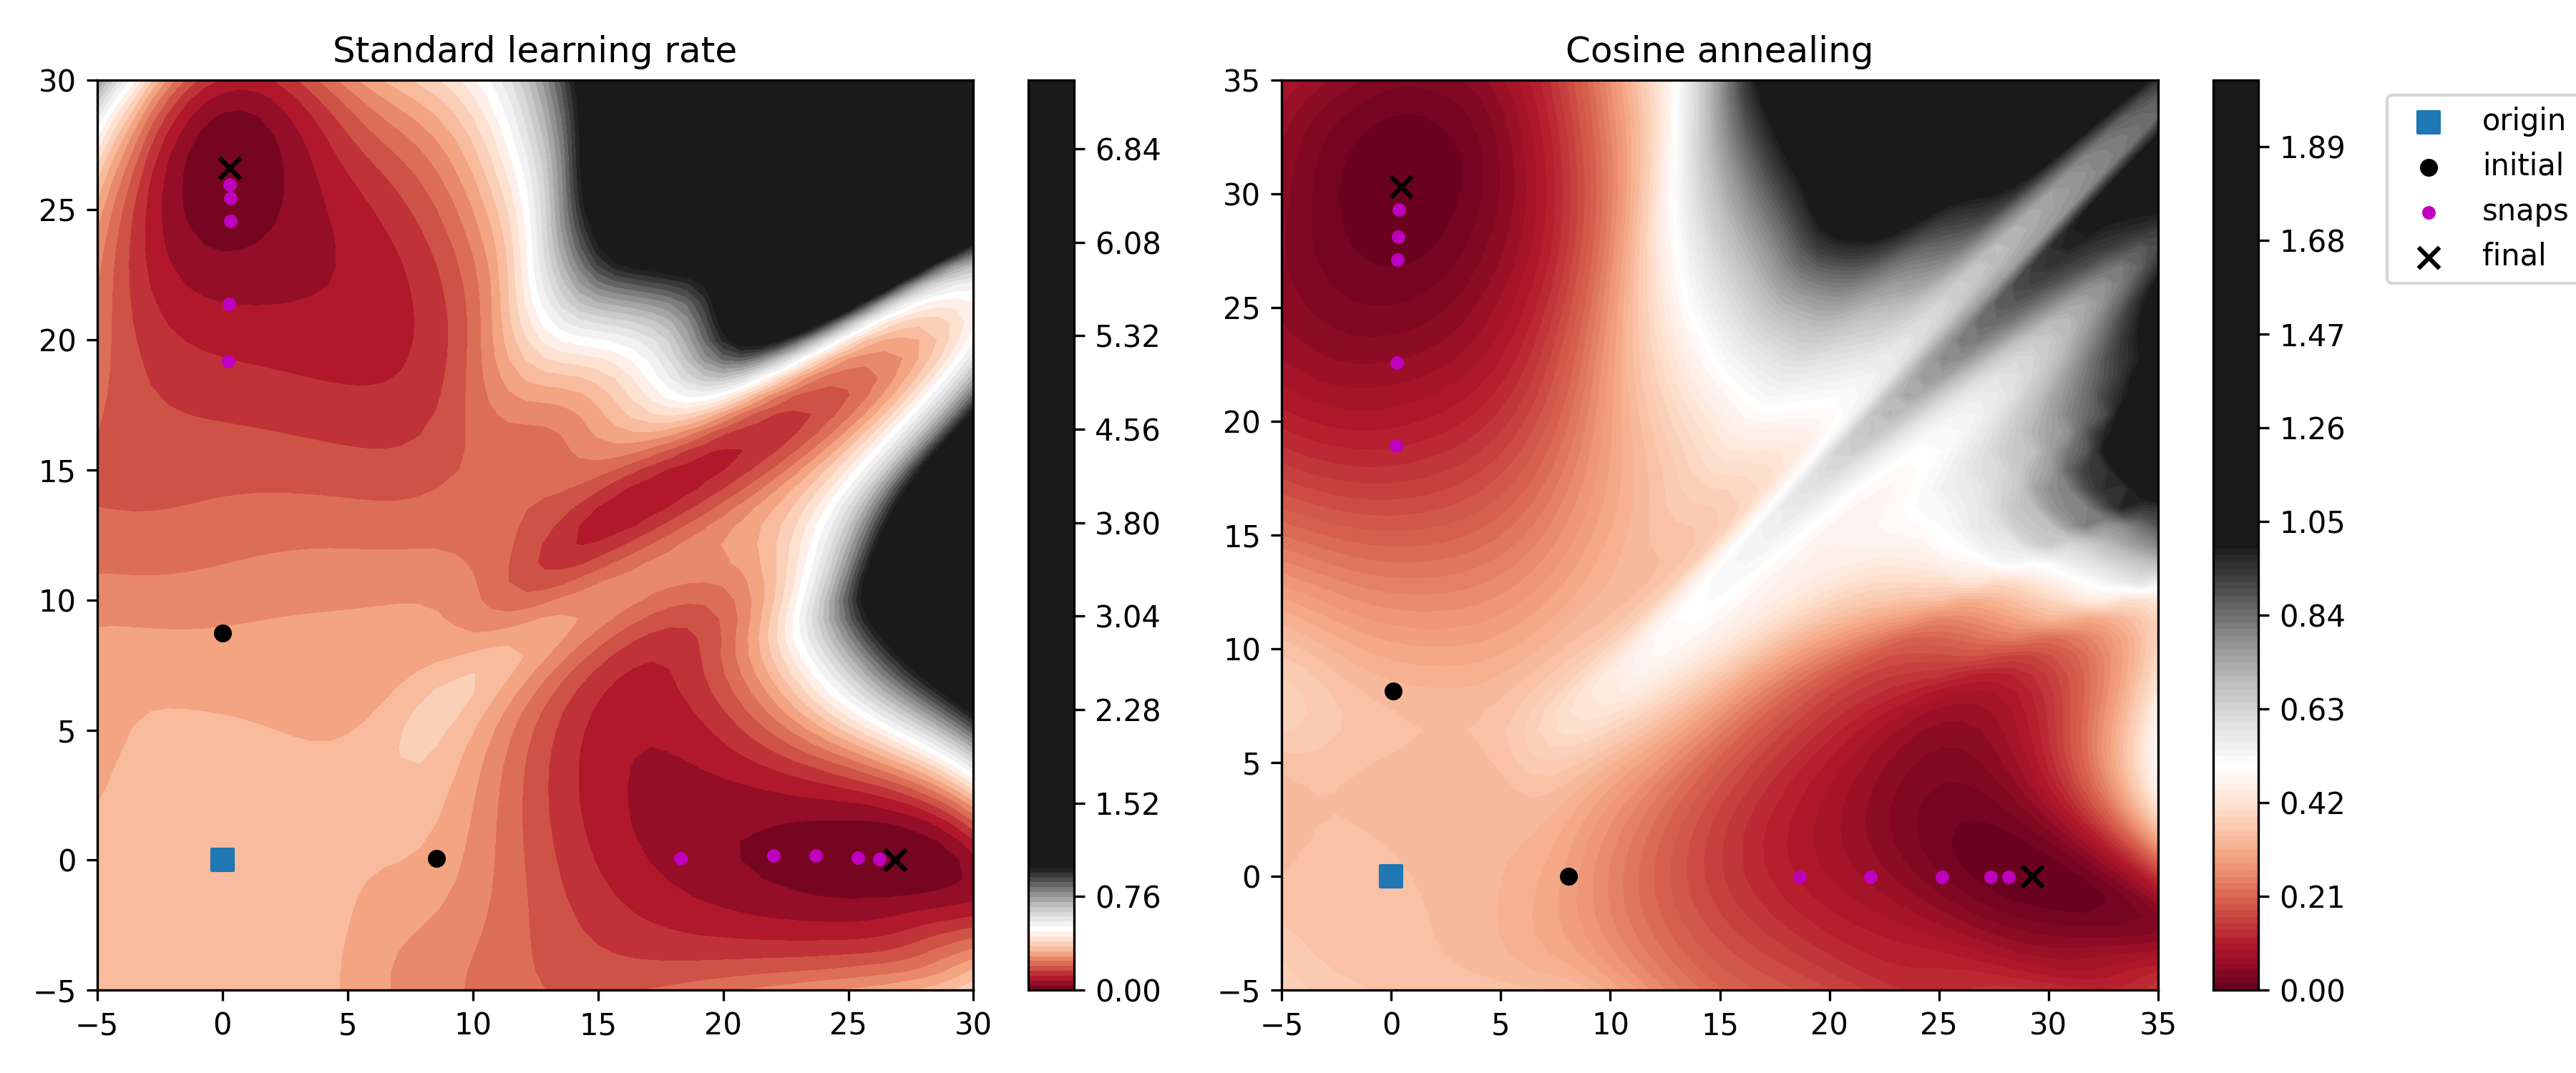
\includegraphics[width=1\linewidth]{./figs/origin_planes.png}  
	\caption{Training loss on the plane defined by the origin (0) and the final parameters from 2 trajectories with different initializations. Earlier snapshots and initial parameters are projected on the plane.}
	\label{}
\end{figure}

\begin{figure}[H]
	\centering
	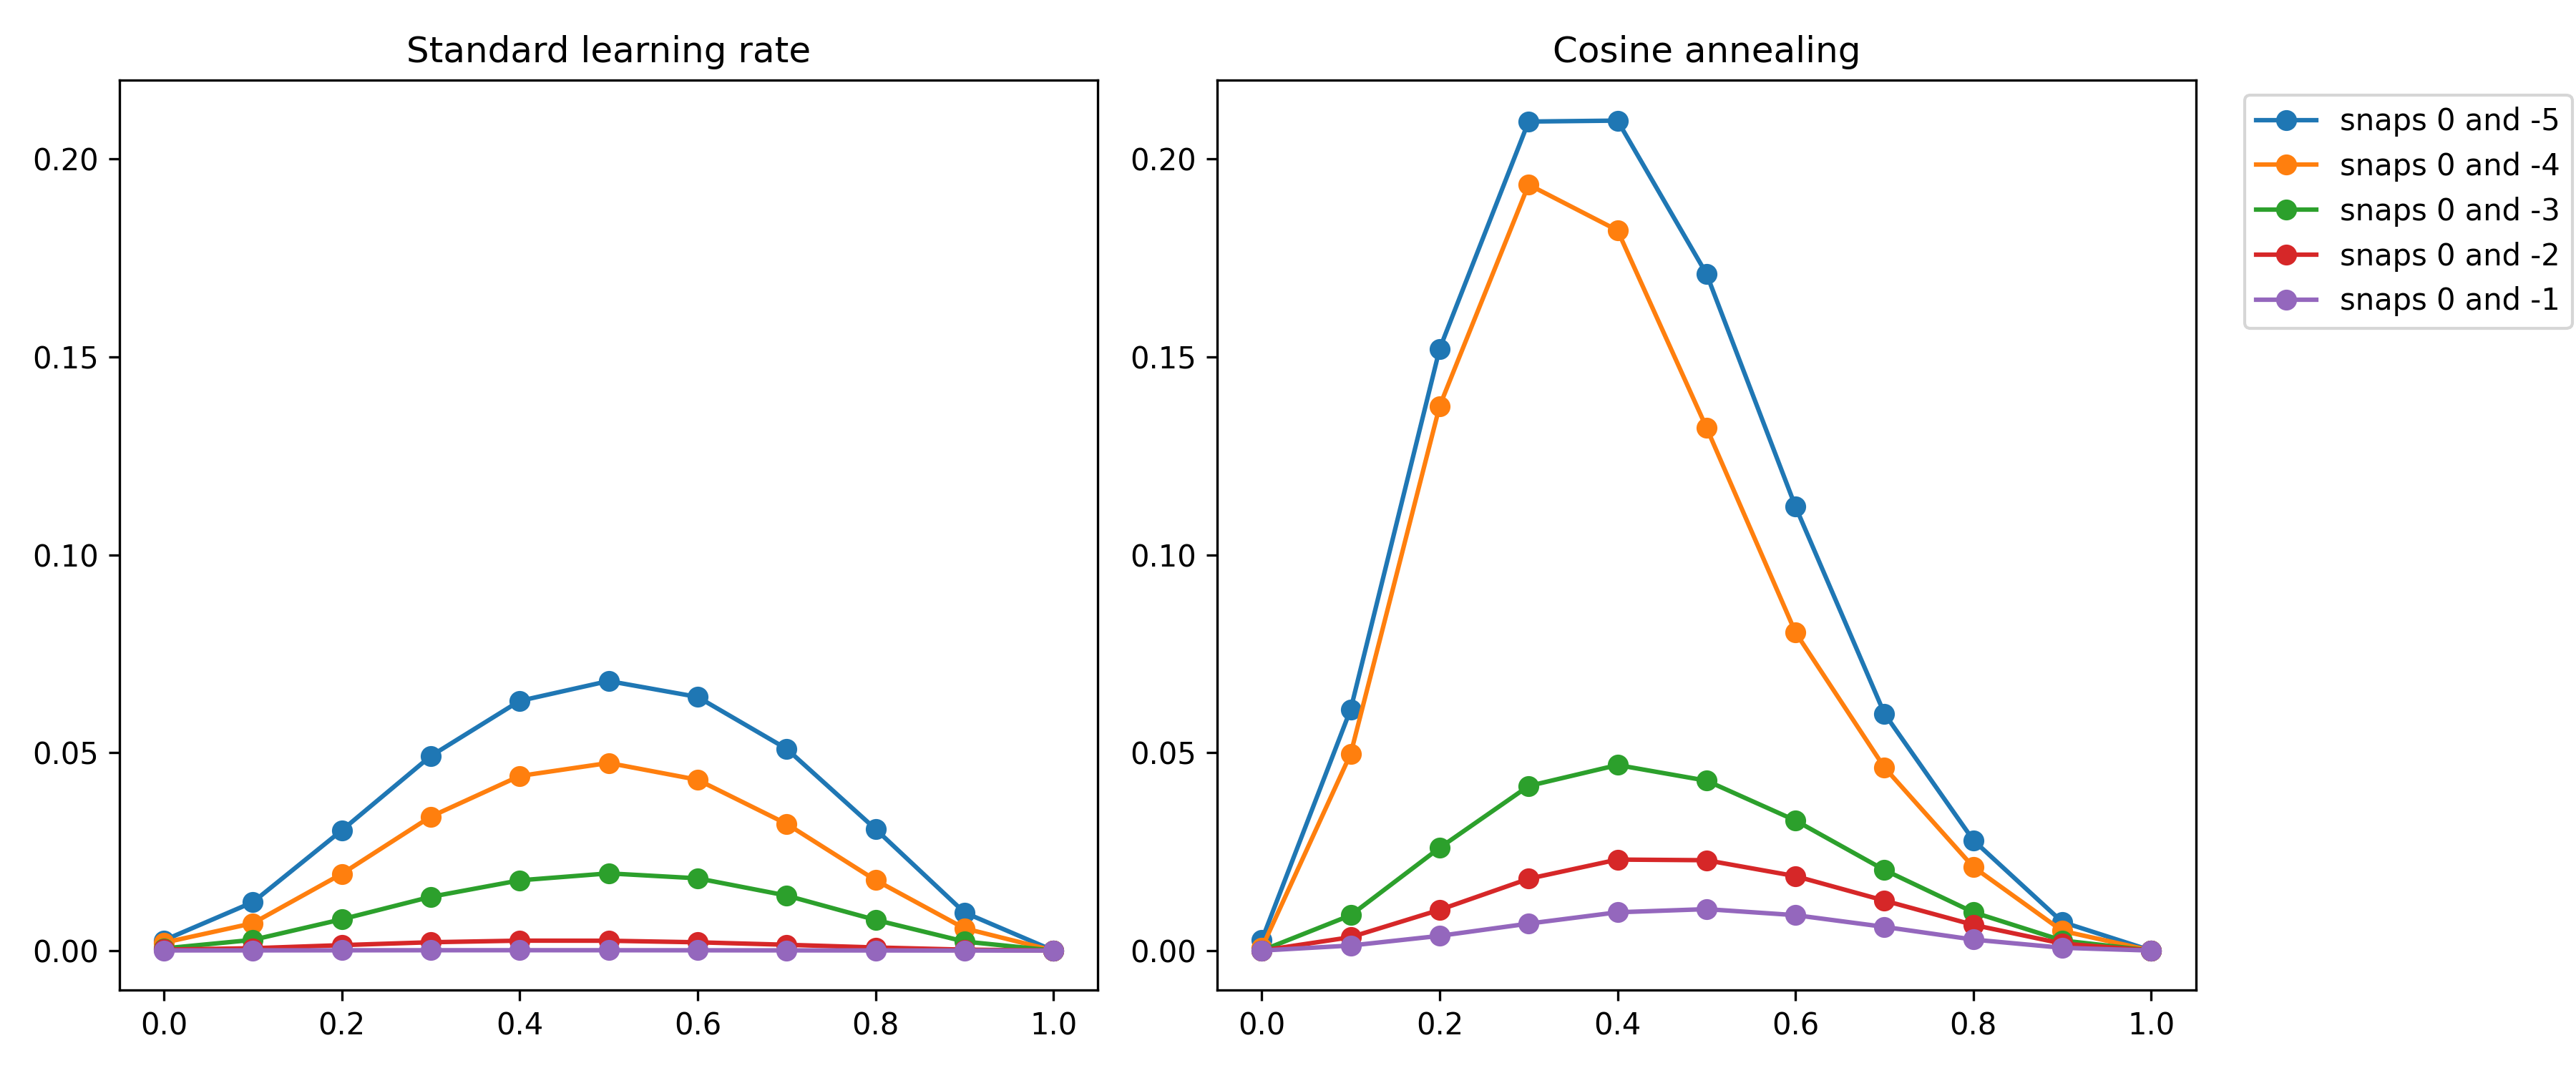
\includegraphics[width=1\linewidth]{./figs/line_plots.png}  
	\caption{Training loss on the line connecting the final parameters from a trajectory and earlier snapshots of that trajectory.}
	\label{}
\end{figure}

\section{What's next for function approximation}
\noindent
\textbf{Make sure the results hold for:}
\begin{itemize}
	\item ``Easier'' functions that are well approximated by a single model.
	\item Different number of datapoints.
	\item Added noise to the data.
\end{itemize}
Also try to evaluate the quality of the obtained uncertainty.

\section{Towards ePINNs?}
\noindent
\textbf{Incorporate to PINNs:}
\begin{itemize}
	\item As it is for better accuracy and for-free uncertainty.
	\item Try to devise a method for active learning while training: resample at high-uncertainty areas.
\end{itemize}
\noindent
\textbf{What I think would be publishable:}
\begin{itemize}
	\item Have 3 techniques: 1 for-free (like snapshot ensembles), 1 with intermediate cost (like scalable MCMC) and a more expensive one (like replica MCMC). 
	\item Compare and discuss applicability for PINNs for big data and large dimensions.
\end{itemize}

%%%%%%%%%%%%%%%%%%%%%%%%%%%%%%%%%%%%%%%%%%%%%%%%%%%%%%%%%%%%%%%%%%%%%%%%%%%%%%%%%%%%%%%%%%%%%%%%%%%%%%%%%	

%\section*{Appendix}
	
\printbibliography[heading=bibintoc,title={References}]
	
\end{document}